\documentclass[12pt,a4paper]{article}
\usepackage[left=3cm,top=2cm,bottom=3cm,right=2cm,includehead,includefoot]{geometry}
\usepackage{amsfonts,amsmath,amssymb,amsthm,graphicx}
\usepackage{answers}
\usepackage[utf8]{inputenc}
\usepackage{german}
\usepackage{ngerman}

\usepackage{pst-pdf}
%\usepackage{wrapfig}
\usepackage{pstricks}
\usepackage{pst-circ}
\usepackage{pst-plot}

\usepackage{booktabs}
\usepackage{microtype}

% Rockt !
%\usepackage{sagetex}

% Muss als letztes eingebunden werden
%\usepackage[bookmarks=true,bookmarksnumbered,colorlinks=true,pdftitle={IPhO-Aufgaben},pdfstartview=FitH,pdfauthor={Pavel Zorin}]{hyperref}
\usepackage[bookmarks=false,pdftitle={IPhO-Aufgabensammlung},pdfstartview=FitH,pdfauthor={Pavel Zorin}]{hyperref}

%Times 10^n
\newcommand{\ee}[1]{\cdot 10^{#1}}
%Units
\newcommand{\unit}[1]{\,\mathrm{#1}}
%Differential d's
\newcommand{\dif}{\mathrm{d}}
\newcommand{\tdif}[2]{\frac{\dif#1}{\dif#2}}
\newcommand{\pdif}[2]{\frac{\partial#1}{\partial#2}}
\newcommand{\ppdif}[2]{\frac{\partial^{2}#1}{\partial#2^{2}}}
%Degree
\newcommand{\degr}{^\circ}

%Degree Celsius (C) symbol
\newcommand{\cel}{\,^\circ\mathrm{C}}

\newcommand{\hinweis}{\emph{Hinweis:} }


%%%%%%%%%%% Aufgaben mit Buchstaben numerieren
\newenvironment{abcenum}{\renewcommand{\labelenumi}{(\alph{enumi})} \begin{enumerate}}{\end{enumerate}\renewcommand{\labelenumi}{\theenumi .}}

%%%%%%%%%% Skizzen %%%%%%%%%%%%
%\newenvironment{skizze}{\begin{wrapfigure}{r}{5.5cm} \vspace{-1cm} \begin{minipage}{5.5cm}}{\end{minipage} }}
\newcommand{\skizze}[1]{
\begin{center}
#1
\end{center}
}


%%%%%%%%%%%%%%%%%%%%%%%%%%%%%%%%%%%%%%%%%%%%%%%%%%%%%%%%%%%%%%%%%%%%%%%%%%%%%%%%%%%%%%%%%%%
%%%%%%%%%%%%%%%%%%%%%%%%%%%%%%%%%%%%%%%%%%%%%%%%%%%%%%%%%%%%%%%%%%%%%%%%%%%%%%%%%%%%%%%%%%%
%
%     Formatierung der Aufgaben/Lösungen
%
%     Anmerkung dazu: nicht-ASCII-Zeichen in Überschriften gehen aus rätselhaften Gründen
%     nicht. Sie werden zwar bei der Aufgabe richtig angezeigt, in die Lösungsdatei wird
%     aber eine unverständliche Sequenz geschrieben, die dann nicht wieder gelesen werden
%     kann.
%
%%%%%%%%%%%%%%%%%%%%%%%%%%%%%%%%%%%%%%%%%%%%%%%%%%%%%%%%%%%%%%%%%%%%%%%%%%%%%%%%%%%%%%%%%%%
%%%%%%%%%%%%%%%%%%%%%%%%%%%%%%%%%%%%%%%%%%%%%%%%%%%%%%%%%%%%%%%%%%%%%%%%%%%%%%%%%%%%%%%%%%%
%\newcommand{aufgabentitel}[1]{\vspace{1cm} {\large\bf \noindent #1} \vspace{.35cm}\\}
\newcounter{numlabel}
\setcounter{numlabel}{0}
%\newenvironment{problem}[2]{\stepcounter{numlabel} \vspace{10ex} {\bf \noindent Aufgabe \the\value{numlabel}: #1 \emph{(#2 Punkte)}} \vspace{1ex}\\ \renewcommand{\Currentlabel}{Aufgabe \the\value{numlabel}: #1}}{
\newenvironment{problem}[2]{\stepcounter{numlabel} \vspace{1ex} \subsubsection*{Aufgabe \the\value{numlabel}: #1 \emph{(#2 Punkte)}} \renewcommand{\Currentlabel}{Aufgabe \the\value{numlabel}: #1}}{

}
\Newassociation{solution}{Soln}{solutions}
\Newassociation{expsolution}{Soln}{expsolutions}
%\renewenvironment{Soln}[1]{\vspace{5ex} {\bf \noindent Lösung zur #1} \vspace{1ex}\\}{
%\renewenvironment{Soln}[1]{\vspace{5ex} {\bf \noindent #1} \vspace{1ex}\\}{
\renewenvironment{Soln}[1]{\subsubsection*{#1}}{

}

\title{IPhO-Aufgabensammlung}
\author{Zusammengestellt von Pavel Zorin\\
unter Verwendung der Aufzeichungen von\\
Bastian Hacker, Igor Gotlibovych und Tobias Holder\\
sowie anonymer Quellen}

\begin{document}
\maketitle

%\frontmatter
Die vorliegende Sammlung umfasst Aufgaben der Klausuren der 3. und 4. Runden der Auswahl zur IPhO aus den Jahren 2006-2008 sowie der 3. Runde 2009.

Die Sammlung ist unter anderem dafür ausgelegt, dass man einen Eindruck von der Schwierigkeit der Klausuren bekommt. Dazu ist bei den theoretischen Aufgaben jeweils die dafür vergebene Punktzahl angegeben. Es hat Klausuren mit 5 bis 8 Aufgaben gegeben, wobei die Gegesamtpunktzahl immer etwa 30 betrug. Die Wahl der Aufgaben wird so getroffen, dass möglichst keine zwei Aufgaben das gleiche Thema aufgreifen. Die Bearbeitungszeit liegt traditionell bei 3 Stunden.

Eine praktische Klausur dauert genauso lange und besteht meist aus einer, seltener aus zwei einfacheren Aufgaben. Typischerweise bringt diese 20 Punkte.

Die 3. und die 4. Runde bestehen jeweils aus 2 theoretischen und 2 praktischen Klausuren, die insgesamt zu erreichende Punktzahl ist also etwa 100.

Die Aufgaben werden nicht offiziell herausgegeben. Deshalb sind die Aufgaben aus dem Gedächtnis niedergeschrieben. Dies bedeutet natürlich, dass die Inhalte nicht unbedingt mit den Originalen übereinstimmen. Insbesondere die Ergebnisse müssen deshalb auch nicht korrekt und vollständig sein.


\section*{Theoretische Aufgaben}

\Opensolutionfile{solutions}[AUTO_LOESUNGSDATEI]

%\subsection*{2006 -- 3. Runde -- Theoretische Klausur I (29.1.06)}

\begin{problem}{Cola mit Eiswuerfel}{3}
Auf einer Party wirft der Gastgeber in Ihr Glas Cola ($m_\mathrm{Cola} = 200\unit{g}$, $T_\mathrm{Cola} = 20\cel$) einen Eiswürfel ($m_\mathrm{Eis} = 40\unit{g}$, $T_\mathrm{Eis} = -1\cel$).
\begin{abcenum}
\item Welche Temperatur hat Ihr Getränk, nachdem das gesamte Eis geschmolzen ist?
\item (Zusatzfrage) Was halten Sie von Ihrem Gastgeber?
\end{abcenum}
Wärmeaustausch mit der Umgebung kann vernachlässigt werden.\\
Die Wärmekapazität von Cola gleicht der des Wassers, $c_{\mathrm{Cola}} = 4200\unit{\frac{J}{kg \cdot K}}$; Wärmekapazität von Eis ist $c_{\mathrm{Eis}} = 2130\unit{\frac{J}{kg \cdot K}}$, latente Schmelzwärme beträgt $3,36\ee{5}\unit{\frac{J}{kg}}$.
\begin{solution}
Der Eiswürfel schmilzt vollständig. Die Endtemperatur beträgt $3,24\cel$
\end{solution}
\end{problem}


\begin{problem}{Licht im Gitter}{4}
Licht von einer Lichtquelle, welche ein festes Linienspektrum 
erzeugt, fällt senkrecht auf ein optisches Gitter mit $300$ Strichen 
pro mm. Unter einem Winkel von $24,46\degr$ beobachtet man Maxima 
für zwei Linien, eine aus dem roten und eine aus dem blauen Bereich des Spektrums.\\
Gibt es andere Winkel, unter denen man Maxima für beide Linien beobachtet?\\
\hinweis\\
rotes Licht: $640\unit{nm}\leq\lambda\leq750\unit{nm}$\\
blaues Licht: $360\unit{nm}\leq\lambda\leq490\unit{nm}$
\begin{solution}
Die rote und die blaue Linie liegen bei $690\unit{nm}$ bzw. $460\unit{nm}$. Die Maxima fallen für\\
$\alpha=0\degr$, $\pm24\degr,46\degr$ und $\pm55,89\degr$ zusammen.
\end{solution}
\end{problem}


\begin{problem}{Amperemeter}{5}
\skizze{
\psset{yunit=0.6366cm}
\psset{xunit=0.9cm}
\begin{pspicture}(-1,-1)(5.5,2.5)
\psline{<->}(0,2)(0,0)(5.2,0)
\uput[l](0,2){$I$}
\uput[d](5.2,0){$t$}
\psline[linewidth=1.5pt](0,1)(5,1)
\uput[r](-1,1){\Large I}
\end{pspicture}

\begin{pspicture}(-1,-1)(5.5,2.5)
\psline{<->}(0,2)(0,0)(5.2,0)
\uput[l](0,2){$I$}
\uput[d](5.2,0){$t$}
\uput[r](-1,1){\Large II}
\psplot[linewidth=1.5pt,plotpoints=400]{0}{5}{x 90 mul sin x 90 mul sin abs add 2 div}
\end{pspicture}

\begin{pspicture}(-1,-1)(5.5,2.5)
\psline{<->}(0,2)(0,0)(5.2,0)
\uput[l](0,2){$I$}
\uput[d](5.2,0){$t$}
\psline[linewidth=1.5pt](0,0)(1,1)(3,-1)(5,1)
\uput[r](-1,1){\Large III}
\end{pspicture}
}
Die abgebildeten Signale I-III werden mit drei verschiedenen Amperemetern gemessen.
Das erste Amperemeter misst den Effektivwert. In allen drei Fällen zeigt es $2\unit{A}$ an.\\
Die Amperemeter 2 und 3 haben Gleichrichter eingebaut (für den gleichgerichteten Strom gilt: $I'=I$ für $I \geq 0$, $I' = 0$ für $I < 0$). Die Anzeige des 2. Amperemeters ist zur Amplitude und die des 3. Amperemeters zum zeitlichen Mittelwert des gleichgerichteten Stroms proportional. Beide Amperemeter sind so geeicht, dass sie bei sinusförmigem Wechselstrom jeweils den Effektivwert anzeigen.\\
Was zeigen die Amperemeter in jedem der Fälle I-III an?
\begin{solution}
% ?
\[
I_{S,I}=2\unit{A},\quad I_{S,II}=\sqrt{2}\cdot 4\unit{A},\quad I_{S,III}=\sqrt{3}\cdot 2\unit{A}
\]
\end{solution}
\end{problem}


\begin{problem}{Flummis}{5}
\skizze{
\psset{unit=0.6cm}
\begin{pspicture}(-2,-0.1)(2,5)
\psline[linewidth=2pt](-1.5,0)(1.5,0)
\pscircle(0,3.7){0.6}\uput{0.9}[l](0,3.7){$m_1$}
\pscircle(0,4.6){0.3}\uput{0.6}[l](0,4.6){$m_2$}
\psline{<->|}(1.2,0)(1.2,4.3)\uput[r](1.2,2){$h$}
\end{pspicture}
}
Zwei Flummis fallen aus einer (großen) Höhe $h$ auf den Boden. Der untere Flummi hat die Masse $m_1$ und der obere $m_2$. Welche Höhe erreicht der obere Flummi nach dem Stoß?\\
Nehmen Sie an, dass alle Stöße elastisch sind.\\
Betrachten Sie den Fall $m_1 > m_2$.\\
Was gilt im Fall $m_1 \gg m_2$?
\begin{solution}
Der obere Flummi erreicht die Höhe $h'=h\left(\frac{3m_1-m_2}{m_1+m_2}\right)^2$. Für $m_1\gg m_2$ ist $h' \approx 9h$.
\end{solution}
\end{problem}


\begin{problem}{Stromdurchflossene Leiterschleife}{5}
\skizze{
\begin{pspicture}(-1,0.5)(4.5,3.5)
\psline[linewidth=1.5pt](0,1)(0,4)
\psline[linewidth=1.5pt]{->}(0,2)(0,3)\uput[l](0,3){$I_0$}
\psframe(1,1.5)(3.5,3.5)
\psline{|<->|}(0,1.3)(1,1.3)\uput[d](0.5,1.3){$d$}
\psline{|<->|}(1,1.3)(3.5,1.3)\uput[d](2.25,1.3){$a$}
\psline{|<->|}(3.7,1.5)(3.7,3.5)\uput[r](3.7,2.5){$b$}
\psline[linewidth=2pt]{->}(2.5,1.5)(3,1.5)\uput[u](2.75,1.5){$I_L$}
\end{pspicture}
}
Eine stromdurchflossene Leiterschleife befindet sich in einer Ebene mit einem stromdurchflossenen
unendlich langen Leiter. Welche Kraft wirkt auf die Leiterschleife?
\begin{solution}
Die auf die horizontalen Leiterabschnitte wirkenden Kräfte heben sich genau auf. Damit reicht es die vertikalen Abschnitte zu betrachten, was eine Integration überflüssig (oder trivial) macht, denn dort ist die Längenkraftdichte konstant. Damit ergibt sich
\[
F=\frac{\mu_0 I_0 I_L b}{2\pi} \left( \frac{1}{d}-\frac{1}{d+a} \right).
\]
Die resultierende Kraft liegt in der Schleifenebene senkrecht zum Leiter, und zeigt vom Leiter weg.
\end{solution}
\end{problem}


\begin{problem}{Herunterfallende Kette}{7}
Eine lose zusammengelegte offene Kette mit der Länge $1\unit{m}$ liegt auf einer Tischkante $1\unit{m}$ über dem Boden. Zum Zeitpunkt $t = 0$ fängt ein Ende der Kette an, reibungslos über die Tisschkante nach unten zu gleiten.\\
Nach welcher Zeit liegen beide Kettenenden auf dem Boden?\\
Nehmen Sie an, dass die Beschleunigung der Kette konstant bleibt, während die Kette über die Tischkante gleitet.
\begin{solution}
Man betrachte zunächst die Phase in der das obere Ende noch auf dem Tisch liegt und bezeichne die Höhe des Tisches und die Länge der Kette mit $h$, die lineare Dichte der Kete mit $\lambda$ und die Länge des bereits fallenden Abschnittes der Kette mit $l$. Impulserhaltung liefert
\[
\lambda l g = \tdif{p}{t}  = \tdif{}{t} (\lambda l l'),
\]
oder umgeschrieben
\[
g l = l l'' + l'^2.
\]
Eine Lösung dieser Gleichung ist
\[
l = \frac a2 t^2, \quad a = \frac g3.
\]
Man sieht leicht dass diese mit den Randbedingungen verträglich ist. $a$ ist die Beschleunigung, die die Kette in dieser Phase erfährt. Diese Phase dauert also
\[
t_1 = \sqrt{\frac{2 h}{a}} = \sqrt{\frac{6 h}{g}}.
\]
Anschließend fällt das obere Ende der Kette frei mit der Beschleunigung $g$ und der Anfangsgeschwindigkeit $a t_1$ die Strecke $h$. Die dafür benötigte Zeit beträgt
\[
t_2 = \frac{-at_1 + \sqrt{a^2 t_1^2 + 2 g h}}{g} = \sqrt\frac{2 h}{3 g}
\]
und die Gesamtzeit damit
\[
t = t_1 + t_2 = \frac{4 \sqrt 6}{3} \sqrt\frac{h}{g} \approx 1,04\unit{s}.
\]
\end{solution}
\end{problem}












%\newpage
%\subsection*{2006 -- 3. Runde -- Theoretische Klausur II (30.1.06)}

\begin{problem}{Temperaturmessung}{3}
\skizze{
\begin{pspicture}(-1.5,-2.8)(3,1)
\pscircle(0,0){1}
\psframe[linecolor=white,fillstyle=solid,fillcolor=white](-0.2,0)(0.2,-1.1) 

\psline[linearc=0.2,linecolor=white,fillstyle=hlines](0.2,-0.98)(0.2,-1.8)(2.1,-1.8)(2.1,-0.98)(2.5,-0.98)(2.5,-2.2)(-0.2,-2.2)(-0.2,-0.98)

\psline[linearc=0.2](0.2,-0.98)(0.2,-1.8)(2.1,-1.8)(2.1,0.7)
\psline[linearc=0.2](-0.2,-0.98)(-0.2,-2.2)(2.5,-2.2)(2.5,0.7)
\psline[linestyle=dashed](-0.2,-0.98)(2.5,-0.98)
\end{pspicture}
}
Eine Glaskugel mit einem Volumen von $7\unit{l}$ ist mit Luft bei einer Temperatur
von $27\cel$ gefüllt. Das anschließende U-förmige Rohr mit einem Querschnitt von $10\unit{cm^2}$
ist mit Quecksilber gefüllt, so dass dessen Höhe in beiden Schenkeln gleich ist. Der Außendruck
beträgt $760\unit{mmHg}$. Die Luft wird nun erwärmt, so dass der Quecksilberspiegel im rechten Rohr
um $5\unit{mm}$ ansteigt.\\
Welche Temperatur hat die Luft in der Kugel?
\begin{solution}
% ?
Die neue Temperatur beträgt $31.2\cel$
\end{solution}
\end{problem}


\begin{problem}{Bremsmanoever}{6}
Eine Raumsonde umkreist mit der Geschwindigkeit $u$ einen Planeten mit Masse $M$.
Während einer sehr kurzen Zeit wird die Sonde um $\Delta u_1$ in Flugrichtung abgebremst.
Im zum Planeten gegenüberliegenden Punkt wird die Sonde nochmals um $\Delta u_2$ abgebremst,
so dass sie sich wieder auf einer Kreisbahn bewegt.
\begin{abcenum}
\item Bestimmen Sie $\Delta u_2$.
\item Bestimmen Sie $u/\tilde u$, wenn $\tilde u$ die Geschwindigkeit auf der neuen Kreisbahn ist. Ist das Verhältnis größer, kleiner oder gleich 1?
\end{abcenum}
\begin{solution}
Energie- und Drehimpulserhaltung:
\[
\Delta u_2=\frac{(u^2+2u\Delta u_1-\Delta u_1^2)-u\sqrt{u^2+2u\Delta u_1-\Delta u_1^2}}{u-\Delta u_1}
\]
\[
\frac{u}{\tilde{u}}=\frac{u-\Delta u_1}{\sqrt{u^2+2u\Delta u_1-\Delta u_1^2}}
\]
Es gilt $u/\tilde u<1$.
\end{solution}
\end{problem}


\begin{problem}{Polarisatoren}{4}
Zwischen zwei um $\frac{\pi}{2}$ gegeneinander verdrehte Polarisatoren werden $k$ ($k=0,1,2...$)
weitere Polarisatoren gestellt, so dass jeder Polarisator gegenüber dem vorigen um
$\frac{\pi}{2(k+1)}$ verdreht ist.\\
Bestimmen Sie den Anteil vom auf den ersten Polarisator einfallenden unpolarisierten Licht,
welcher durch das System durchgelassen wird.\\
Betrachten Sie insbesondere die Grenzfälle.
\begin{solution}
\[
\alpha=\frac{1}{2}\left( \cos^2\frac{\pi}{2(k+1)} \right)^{k+1}
\]
\[
k=0 \implies \alpha=0
\]
\[
k\to\infty \implies \alpha=\frac{1}{2}
\]
\end{solution}
\end{problem}


\begin{problem}{Manipulation von Elektronen}{5}
\skizze{
  \begin{pspicture}(-0.5,-1.5)(5,1.5)
\psline{->}(0,-1.3)(0,1.3)\uput[l](0,1){$\rho$}
\psline{->}(-0.2,0)(4.5,0)\uput[d](4.5,0){$x$}
\psplot[linewidth=0.5pt,plotpoints=400, arrows=->]{1}{3.5}{1 x sqrt div}\uput[ur](2,0.7){$- \vec{E}$}
\psplot[linewidth=0.5pt,plotpoints=300, arrows=->]{0.25}{3.5}{0.5 x sqrt div}
\psplot[linewidth=0.5pt,plotpoints=200, arrows=->]{0.0625}{3.5}{0.25 x sqrt div}
\psplot[linewidth=0.5pt,plotpoints=100, arrows=->]{0.015625}{3.5}{0.125 x sqrt div}
\psplot[linewidth=0.5pt,plotpoints=100, arrows=->]{0.015625}{3.5}{0.125 neg x sqrt div}
\psplot[linewidth=0.5pt,plotpoints=200, arrows=->]{0.0625}{3.5}{0.25 neg x sqrt div}
\psplot[linewidth=0.5pt,plotpoints=300, arrows=->]{0.25}{3.5}{0.5 neg x sqrt div}
\psplot[linewidth=0.5pt,plotpoints=400, arrows=->]{1}{3.5}{1 neg x sqrt div}
\psline[linewidth=0.5pt]{|-|}(3.8,0)(3.8,0.3)\uput[r](3.8,0.15){$r$}
\end{pspicture}
}
\begin{abcenum}
\item Elektronen durchlaufen eine Beschleunigungsspannung von $U_\mathrm{B}$ und kommen dann
unter einem Winkel $\varphi$ durch das Loch in einer der Platten in das Feld eines Plattenkondensators,
an dem eine Spannung $U_\mathrm{K}$ anliegt.\\
Welche Geschwindigkeit hat das Elektron, wenn es durch ein zweites Loch den Kondensator wieder verlässt?
\item In einem bestimmten ladungsfreien Bereich herrscht ein radialsymmetrisches elektrisches Feld. Die $x$-Komponente des Feldes hängt dabei nur von $x$ ab und beträgt $E_x(x) = -2 a x$ mit $a=2\ee{6}\unit{V/m^2}$. Man bestimme die Radialkomponente des Feldes im achsennahen Bereich und insbesondere im Abstand $r=3\unit{mm}$ von der $x$-Achse.
\end{abcenum}

\begin{solution}
\begin{abcenum}
\item Die Geschwindigkeit beträgt (nicht-relativistisch) $\sqrt{\frac{2e(U_\mathrm{B}+U_\mathrm{K})}{m}}$, falls das Elektron die gegen\-über\-liegende Platte erreicht, und $\sqrt{\frac{2eU_\mathrm{B}}{m}}$, falls das Elektron im Kondensator umkehrt und wieder durch die gleiche Platte geht. Dies ist für $\cos\varphi<\sqrt{\frac{U_\mathrm{K}}{U_\mathrm{B}}}$
der Fall, falls das $U_\mathrm{K}$ so anliegt, dass die Platte, durch die das Elektron eintritt, positiv geladen ist.\\
\item Divengenzfreiheit des statischen elektrischen Feldes in Abwesenheit von Ladungen liefert
\[
0 = \nabla \vec E = \pdif{}{x} E_x + \frac1\rho \pdif{}{\rho} (\rho E_\rho) = -2 a + E_\rho' + \frac{1}{\rho} E_\rho.
\]
Die Lösung dieser Gleichung mit $E_\rho \to 0$ bei $\rho \to 0$ ist $E_\rho(\rho) = a \rho$, die exakte Lösung stimmt also mit der achsennahen Näherung überein. Im Abstand $r$ bekommt man schließlich
\[
E_\rho(r)=6\ee{3}\unit{V/m}.
\]
\end{abcenum}
\end{solution}
\end{problem}


\begin{problem}{Ionisiertes Helium}{6}
Das ionisierte Helium He$^+$ verhält sich wasserstoffähnlich. Es hat die Energieniveaus
$-\frac{54,4\unit{eV}}{n^2}$ mit $n=(1,2,\ldots)$. Ein He$^+$-Gas wird aus einer bestimmten Richtung
mit Licht der Wellenlängen $24\unit{nm}\leq\lambda\leq50\unit{nm}$ bestrahlt.
\begin{abcenum}
\item Wie viele Absorptionslinien sieht man, wenn man entgegen der Strahlungsrichtung blickt? Welche Wellenlängen haben sie?
\item Welche Emissionslinien beobachtet man entgegen bzw. senkrecht zur Strahlungsrichtung?
\end{abcenum}
\begin{solution}
\begin{abcenum}
\item Man sieht 3 Absorbtionslinien: $24,3\unit{nm}$, $25,6\unit{nm}$, $30,4\unit{nm}$
\item senkrecht 6 Emissionslinien: $24,3\unit{nm}$, $25,6\unit{nm}$, $30,4\unit{nm}$, $121,6\unit{nm}$, $164,1\unit{nm}$, $468,9\unit{nm}$, entgegen: die selben, außer die von (a)
\end{abcenum}
\end{solution}
\end{problem}


\begin{problem}{Fallender Magnet}{7}
Ein Stabmagnet mit dem magnetischen Moment $\mu$ fällt mit dem Nordpol nach unten in einem engen isolierenden Zylinder. Um diesen herum befindet sich ein zweiter isolierender Zylinder mit dem Radius $r$, auf dem in regelmäßigen Abständen $h$ Leiterschleifen aufgewickelt sind, die einen Widerstand von je $R$ haben. Der Magnet hat die Masse $m$ und erreicht nach kurzer Zeit eine konstante Geschwindigkeit $v$, die von $m$, $\mu$, $h$, $R$, $r$, $\mu_0$ abhängt.\\
Wie ändert sich $v$, wenn man jeweils eine der Größen $m$, $\mu$, $h$, $R$, $r$ verdoppelt und die anderen dabei konstant lässt?\\
Die Luftreibung, das Erdmagnetfeld sowie Selbst- und Gegeninduktion der Leiterschleifen können vernachlässigt werden.
\begin{solution}
Die Änderung von $v$ durch die Parameter lässt sich mit einer Einheitenanalyse bestimmen.
\[
\Rightarrow\qquad v \sim \frac{m\cdot g\cdot h\cdot R \cdot r^3}{\mu^2\cdot \mu_0^2}
\]
Alternativ kann man auch die vertikale Komponente des Magnetfeldes des Stabmagneten $B_z(z,r)$ bestimmen, dann hat man für die Spannung an einem Ring im Abstand $z$ vom Magneten
\[
U(z) = \tdif{}{t} \int\limits_{\rho \leq r} B(z,\rho) \dif A = v \tdif{}{z} \int\limits_{\rho \leq r} B(z,\rho) \dif A
\]
Wenn man nun eine Zeit $\Delta t = h/v$ und die zugehörigen Energieverluste an allen Leiterschleifen betrachtet, bekommt man
\[
\Delta E = \sum_{i=-\infty}^{+\infty} \int\limits_{t=0}^{\Delta t} \frac{U^2(z_i(t))}{R} \dif t
= \frac{1}{Rv} \int\limits_{z=-\infty}^{+\infty} U^2(z) \dif z = mgh
\]
Es reicht dann bei $\Delta E$ einen der Terme (sinnvollerweise den einfachsten) zu integrieren um die Exponenten der Parameter zu bekommen.

\end{solution}
\end{problem}













%\newpage
%\subsection*{2006 -- 4. Runde -- Theoretische Klausur I (19.4.06)}

\begin{problem}{Masse des Seils}{3}
\skizze{
\psset{unit=1cm}
\begin{pspicture}(-0.5,-1)(5,3.8)
\psline[linewidth=0pt,linecolor=white,fillstyle=hlines](-0.4,-0.5)(0,-0.5)(0,3.8)(-0.4,3.8)
\psline[linewidth=1pt](0,-0.5)(0,3.8)
\psplot[linewidth=1.5pt,plotpoints=400,arrows=*-|]{0}{4}{2 x 4 sub 0.498 mul exp 2 x 4 sub neg 0.498 mul exp add 2 sub 0.69 div}
\psline{->, linewidth=2.5pt}(4,0)(5,0)\uput[u](4.5,0){$F$}
\end{pspicture}
}
Ein homogenes flexibles Seil ist fest an einer Wand aufgehängt. Es wird von einer Kraft $F=20\unit{N}$ in horizontaler Richtung gehalten und hängt dabei in Ruhe. Die Skizze ist maßstabsgetreu und darf für Berechnungen verwendet werden.\\
Wie groß ist dann die Masse des Seiles?


\begin{solution}
Winkel an der Wand $\alpha\approx28\degr$.
\[
m=\frac{20\unit{N}}{g\cdot\tan{\alpha}}\approx3,8\unit{kg}
\]
\end{solution}
\end{problem}


\begin{problem}{Beschichtete Glasplatte}{4}
Eine dicke Glasplatte $(n=1,5)$ ist mit einer dünnen Folie $(n=1,3)$ beschichtet und befindet sich in Luft. Abgebildet ist das Transmissionsspektrum bei senkrechtem Einfall von Strahlung:\\
\begin{center}
\psset{xunit=0.05cm,yunit=0.04cm}
\begin{pspicture}(-20,-20)(185,120)
\psaxes[arrows=->,Ox=480,Dx=20,dx=20,Dy=20,dy=20,ticksize=0.04](0,0)(0,0)(160,115)
\uput[dr](160,0){$f$, $\unit{THz}$}\uput[l](0,115){$I$}
%\psplot[linewidth=0.5pt,plotpoints=2000]{0}{150}{x 5 mul sin 30 mul x 100 mul sin 8 mul add 40 add}
\psplot[linewidth=0.8pt,plotpoints=2000]{0}{150}{
48
x 12 div sub
6.76 x mul 9.45 add cos 10 mul sub
2.58 x mul cos 20 mul sub
0.4 x x mul mul 90 x mul add cos 5 mul sub}
\end{pspicture}
\end{center}
Bestimmen Sie die Dicke der Folie!
\begin{solution}
% ?
etwa $50\unit{\mu m}$ (zumindest die Größenordnung sollte stimmen)
\end{solution}
\end{problem}


\begin{problem}{Draht im homogenen Gravitationsfeld}{4}
Ein homogener Draht der Dichte $\rho$ mit maximaler Zugspannung $\sigma$ hängt im homogenen Schwerefeld der Stärke $g$. Am Aufhängepunkt besitzt der Draht den Radius $r_0$, und sein Querschnitt ist überall kreisförmig.\\
Welche Form muss der Draht haben, wenn er überall bis zur maximalen Belastung gespannt sein soll?
\begin{solution}
\[
r(x)=r_0\cdot \exp\left( -\frac{\rho g}{2\sigma}\cdot x\right)
\]
\end{solution}
\end{problem}


\begin{problem}{Fette Robbe}{5}
Eine Robbe (Länge $1,5\unit{m}$, Umfang $1,5\unit{m}$) befindet sich im Wasser bei $0\cel$. Die Robbe besitzt eine Wärmeleistung von $100\unit{W}$ und eine Körpertemperatur von $37\cel$. Sie ist mit einer Fettschicht mit dem Wärmeleitungskoeffizienten $\lambda = 0,14\unit{\frac{W}{m\cdot K}}$ umgeben.\\
Schätzen Sie die Dicke der Fettschicht ab, und geben dabei alle gemachten Näherungen an.
\begin{solution}
\skizze{
\psset{unit=1cm}
\begin{pspicture}(0,0)(4,1)
\psline[linewidth=1pt](0.477,0)(2.523,0)
\psline[linewidth=1pt](0.477,0.955)(2.523,0.955)
\psarc[linewidth=1pt]{-}(0.477,0.477){0.477}{90}{270}
\psarc[linewidth=1pt]{-}(2.523,0.477){0.477}{270}{90}
\psellipticarc[linewidth=1pt]{-}(0.477,0.477)(0.2,0.477){90}{270}
\psellipticarc[linewidth=1pt,linestyle=dashed,dash=2pt 4pt]{-}(0.477,0.477)(0.2,0.477){270}{90}
\psellipticarc[linewidth=1pt]{-}(2.523,0.477)(0.2,0.477){90}{270}
\psellipticarc[linewidth=1pt,linestyle=dashed,dash=2pt 3pt]{-}(2.523,0.477)(0.2,0.477){270}{90}
\psline[linewidth=0.5pt,linestyle=dashed,dash=2pt 2pt](0.477,0.175)(2.523,0.175)
\psline[linewidth=0.5pt,linestyle=dashed,dash=2pt 2pt](0.477,0.780)(2.523,0.780)
\psarc[linewidth=0.5pt,linestyle=dashed,dash=2pt 2pt]{-}(0.477,0.477){0.302}{90}{270}
\psarc[linewidth=0.5pt,linestyle=dashed,dash=2pt 2pt]{-}(2.523,0.477){0.302}{270}{90}
\psellipse[linewidth=0.5pt,linestyle=dashed,dash=2pt 2pt](0.477,0.477)(0.1,0.302)
\psellipse[linewidth=0.5pt,linestyle=dashed,dash=2pt 2pt](2.523,0.477)(0.1,0.302)
\end{pspicture}
}
Beispiel: Zylinder mit Halbkugeln. $O_0=2,25\unit{m^2}$
\[
\int_{r_0-d}^{r_0}\frac{\dif r}{O(r)}=\frac{\lambda\cdot\Delta T}{P}
\qquad\Rightarrow\qquad
d\approx 9\unit{cm}
\]
\end{solution}
\end{problem}


\begin{problem}{Stromstaerke}{6}
In einem sehr großen Plattenkondensator mit Plattenabstand $d=1\unit{cm}$ befindet sich in einer Platte ein kleines Loch, durch das ein Laserstrahl der Wellenlänge $405\unit{nm}$ senkrecht eintritt. Auf der gegenüberliegenden Platte werden dadurch Elektronen energetisch angeregt. Nach dem Überwinden der Ablösearbeit $1,87\unit{eV}$ fliegen die Elektronen mit gleicher Wahrscheinlichkeit in alle Richtungen. Am Kondensator liegt eine Spannung $U$ an.
\begin{abcenum}
  \item Berechnen Sie den Strom zwischen den beiden Platten in Abhängigkeit von $U$.
  \item Was geschieht qualitativ, wenn man
  \begin{enumerate}
    \item die Annahme wegfallen lässt, dass alle Elektronen die gleiche Energie besitzen?
    \item die endlichen Ausmaße des Kondensators berücksichtigt?
  \end{enumerate}
\end{abcenum}
\begin{solution}
% ?
\[
E=\frac{h\cdot c}{\lambda}-1,87\unit{eV}=1,19\unit{eV}, \quad E_y=1,19\unit{eV}\cdot \cos^2\alpha
\]
Raumwinkelanteil:
\[
\frac{\Omega}{2\pi} = 1-\cos{\alpha} \implies I=I_0\cdot\left(1-\sqrt{\frac{U}{1,19\unit{V}}}\right)
\]
\end{solution}
\end{problem}


\begin{problem}{Strahl und Spiegel}{6}
\skizze{
\psset{unit=1.1cm}
\begin{pspicture}(-1,0)(3,2.5)
\psline[linewidth=0pt,linestyle=none,fillstyle=hlines](1.4,0.6)(0,2)(0,1.6)(1.2,0.4)
\psline[linewidth=1pt](2,0)(0,2)
\psline[linewidth=1pt,linestyle=dashed](1,1)(2,2)
\psline[linewidth=1pt,arrows=-](1.2,2.5)(1,1)
\psline[linewidth=1pt,arrows=->](1.2,2.5)(1.15,2.125)
\psline[linewidth=1pt,arrows=->](1,1)(2.5,1.4)
\psline[linewidth=1pt,linestyle=dashed](0,0)(3,0)
\psarc{-}(2,0){0.8}{135}{180}\uput[ul](1.7,0){$\theta$}
\psarc{-}(1,1){0.9}{45}{82.4}\uput[ur](1.05,1.4){$\alpha$}
\psarc{-}(1,1){1}{14.9}{45}\uput[r](1.3,1.3){$\beta$}
\psline[linewidth=1.5pt,arrows=->](-0.2,0.7)(0.5,0.7)\uput[u](0.15,0.7){$v$}
\end{pspicture}
\psset{unit=1.1cm}
\noindent\begin{pspicture}(-1,-0.1)(3,2.8)
\psline[linewidth=0pt,linestyle=none,fillstyle=hlines](1,0.7)(1,2.5)(0.7,2.5)(0.7,0.7)
\psline[linewidth=1pt](1,0)(1,2.5)
\psline[linewidth=1pt,linestyle=dashed](1,1.3)(2.5,1.3)
\psline[linewidth=1pt,arrows=-](2.3,2.05)(1,1.3)
\psline[linewidth=1pt,arrows=->](2.3,2.05)(2,1.8625)
\psline[linewidth=1pt,arrows=->](1,1.3)(2.3,0.21)
\psline[linewidth=1pt,linestyle=dashed](0,0)(3,0)
\psarc{-}(1,0){0.65}{90}{180}\uput[ul](1.1,0){$90^\circ$}
\psarc{-}(1,1.3){1.1}{0}{30}\uput[ur](1.5,1.3){$\alpha$}
\psarc{-}(1,1.3){1}{-40}{0}\uput[dr](1.5,1.3){$\beta$}
\psline[linewidth=1.5pt,arrows=<-](-0.2,1)(0.5,1)\uput[u](0.15,1){$v$}
\end{pspicture}
}
Ein Spiegel bewegt sich wie in der Skizze mit relativistischer Geschwindigkeit. Es lässt sich zeigen, dass dabei folgende Beziehung gilt:
\[
\sin{\alpha}-\sin{\beta}=\frac{v}{c}\cdot \sin{\theta}\cdot \sin{(\alpha + \beta)}
\]
\begin{abcenum}
\item Man zeige ohne Verwendung der Lorentz-Transformation, dass dann in folgender Skizze die Beziehung gelten muss:
\[
\cos \beta = \frac{(1+(\frac{v}{c})^2)\cos \alpha -2\frac{v}{c}}{1-2\frac{v}{c}\cos \alpha + (\frac{v}{c})^2}
\]
\item Entsprechend der 2. Skizze mit $v=0.6 c$ fällt Laserlicht der Frequenz $f$ unter einem Winkel von $\alpha=30^\circ$ ein. Wie groß ist dann die Frequenz des reflektierten Strahls, und wie groß ist die relative änderung $\frac{\Delta f}{f}$?
\end{abcenum}

\begin{solution}
% ?
\[
f' \approx 0.505 f, \qquad \frac{\Delta f}{f} \approx 49.5\,\%
\]
\end{solution}
\end{problem}











%\newpage
%\subsection*{2006 -- 4. Runde -- Theoretische Klausur II (21.4.06)}

\begin{problem}{Kondensatoren}{3}
Zwei identische Plattenkondensatoren der Kapazität $C$ sind parallel geschaltet. Dabei befindet sich eine Platte des ersten Kondensators zu $\frac{2}{3}$ in der Mitte des zweiten. Die Flächen der Kondensatoren dürfen als groß angenommen und Randeffekte vernachlässigt werden.\\
Wie groß ist dann die Kapazität der Schaltung?
\begin{solution}
\[
C_\mathrm{neu}=\frac{1}{3}C+\frac{2}{3}\cdot 2\cdot C+\frac{1}{3}C=2C
\]
\end{solution}
\end{problem}


\begin{problem}{Variierende Objektgroesse}{3}
Eine kurzsichtige Person sieht ein kleines Objekt und nimmt ihre Brille ab. Sobald sie die Brille langsam zum Objekt hinbewegt, erscheint dieses immer kleiner. Bei einem bestimmten Abstand erscheint das Objekt am kleinsten, bei weiterer Annäherung der Brille scheint es wieder größer zu werden.\\
Bei welchem Abstand der Brille zum Objekt erscheint dieses am kleinsten?
\begin{solution}
% ?
Die Brille ist eine Streulinse mit Brennweite $f$;\qquad $g$ und $b$ sind auf die Augenlinse bezogen.
\[
\frac{B}{G}=\frac{b f}{g(x+f)-x^2}
\]
\[
\tdif{}{x}\frac{B}{G}=\frac{b f\cdot (2x-g)}{(g(x+f)-x^2)^2}=0
\]
\[
x=\frac{g}{2}
\]
\end{solution}
\end{problem}


\begin{problem}{Magnetische Induktion}{3}
An einem regelmäßigen geschlossenem Sechseck aus einem homogenen dünnen Draht liegt an zwei benachbarten Ecken eine Spannung an.\\
Wie groß ist das Magnetfeld $\vec{B}$ in Betrag und Richtung, welches im Mittelpunkt des Sechsecks induziert wird?\\
Der Einfluss der Zuleitungen darf dabei vernachlässigt werden. Führen Sie, wenn nötig, geeignete Variablen ein.
\begin{solution}
\[
\vec{B}=\vec{0}\unit{T}
\]
\end{solution}
\end{problem}


\begin{problem}{Rotierende Scheibe mit Auflage}{4}
\skizze{
\begin{pspicture}(-3,-1)(2.5,1.5)
\psline[linewidth=1pt](-2.5,0)(2.5,0)
\psline[linewidth=0.75pt,linestyle=dashed](0,0.27)(0,1.5)
\psellipticarc[linewidth=1pt]{->}(0,0.93)(0.4,0.2){120}{65}\uput[r](0.4,1){$\omega$}
\pspolygon[linewidth=1pt](-2,0)(-0.8,0)(-0.8,0.4)(-2,0.4)\uput[u](-1.4,-0.1){$M$}
\pscircle[linewidth=1pt](-0.1,0.1){0}
\pscircle[linewidth=1pt](-0.1,0.1){0.1}
\psline[linewidth=0.5pt](-0.8,0.2)(-0.1,0.2)
\psline[linewidth=0.5pt](0,0.1)(0,-0.6)
%\psarc[linewidth=0.5pt]{-}(-0.1,0.1){0.1008775}{0}{90}
\pspolygon[linewidth=1pt](-0.3,-1)(0.3,-1)(0.3,-0.6)(-0.3,-0.6)\uput[u](0,-1.05){$m$}
\end{pspicture}
}
Ein dünner Stab mit Länge $d$ und Masse $M$ liegt in radialer Richtung auf einem ebenen horizontalen Teller, der sich mit $\omega$ um seine vertikale Achse dreht. An dem Stab ist ein masseloser Faden befestigt, an dem ein Gewicht der Masse $m$ hängt. Zwischen Stab und Tisch herrscht der Reibungsfaktor $f$.\\
In welchen Entfernungen von der Drehachse darf der Stab liegen, damit er sich nicht bewegt?
\begin{solution}
\[
\frac{g}{\omega^2}\left(\frac{m}{M}-f\right)-\frac{d}{2}\quad\leq\quad x
\quad\leq\quad\frac{g}{\omega^2}\left(\frac{m}{M}+f\right)-\frac{d}{2}
\]
\end{solution}
\end{problem}


\begin{problem}{Druckbetrachtungen}{5}
In einem Zylinder mit Kolben befindet sich ein ideales Gas ($\kappa=\frac{7}{5}$) unter dem Druck $p_1$. Das Gas wird nun adiabatisch bis zum Druck $\tilde{p}$ komprimiert. Daraufhin wird es isobar abgekühlt bis zu der Temperatur, die es am Anfang hatte. Danach wird weiter adiabatisch komprimiert bis zum Druck $p_2$.\\
Wieviel Energie braucht man dafür?\\
Wie muss $\tilde{p}$ gewählt werden, damit die Arbeit minimal wird?
\begin{solution}
\[
\Delta W =\frac{p_1\cdot V_1}{\kappa-1}\cdot\left(\left(\frac{\tilde{p}}{p_1}\right)^{1-\frac{1}{\kappa}} +\left(\frac{p_2}{\tilde{p}}\right)^{1-\frac{1}{\kappa}}-2\right)
\]
\[
\tilde{p} = \sqrt{p_1\cdot p_2}
\]
\end{solution}
\end{problem}

\begin{problem}{Zerfalendes Proton}{4}
Nach einer Theorie ist es möglich, dass ein Proton spontan in ein Meson und ein Positron zerfällt. Die Wahrscheinlichkeit ist äußerst gering, jedoch von $0$ verschieden. Um das zu überprüfen, hat man Tanks aufgebaut, die mit $3.3\ee{3}\unit{t}$ reinem Wasser gefüllt sind. An den Tanks sind Detektoren angebracht, die jeden Zerfall registrieren. Schätzen Sie die Halbwertszeit des Zerfalls ab, wenn innerhalb eines Jahres kein einziger Zerfall registriert wurde. Wie groß ist die Halbwertszeit, wenn innerhalb eines Jahres mit $95\%$ Wahrscheinlichkeit mindestens ein Proton zerfällt?
\begin{solution}
% ?
Die Anzahl der Protonen beträgt
\[
N=\frac{10}{18}\cdot\frac{3.3\ee{3}\unit{t}}{1u}\approx 1.1\ee{33}.
\]
\end{solution}
\end{problem}


\begin{problem}{Bewaesserungsanlage}{4}
\skizze{
\begin{pspicture}(-2.75,-1.7)(2.75,1)
\psline[linewidth=1pt](-1.5,0)(-1,0)
\psline[linewidth=1pt](-1,0)(-0.1,-0.9)(-0.1,-1.2)
\psline[linewidth=1pt](0.1,-1.2)(0.1,-0.9)(1,0)
\psline[linewidth=1pt](1,0)(1.5,0)
\psline[linewidth=1pt,arrows=->](0,-1.6)(0,-1.2)
\psarc[linewidth=1pt,linestyle=dashed]{-}(0,-1){1.414}{45}{135}
\psline[linewidth=0.5pt,arrows=->](-0.89,0.33)(-1.11,0.66)
\psline[linewidth=0.5pt,arrows=->](-0.31,0.57)(-0.39,0.96)
\psline[linewidth=0.5pt,arrows=->]( 0.31,0.57)( 0.39,0.96)
\psline[linewidth=0.5pt,arrows=->]( 0.89,0.33)( 1.11,0.66)
\psline[linewidth=0.5pt](0,-0.5)(0,0.414)
\psline[linewidth=0.5pt](-0.4,-0.307)(-0.6,0.039)
\psarc[linewidth=1pt]{-}(0,-1){1}{90}{120}\uput[l](0.1,-0.3){$\alpha$}
\end{pspicture}
}
Eine Bewässerungsanlage besteht aus einem hohlen kugelsegmentförmigen Kopf, in den von unten Wasser gepumpt wird. In der oberen Schale befinden sich fein verteilte Löcher, durch die das Wasser überall gleich schnell ausströmt. Die lokale Lochdichte $\rho$ soll überall so groß sein, dass die Rasenfläche gleichmäßig beregnet werden kann. Das Kugelsegment hat einen Öffnungswinkel von $90\degr$ und darf als sehr klein angenommen werden.\\
Wie muss dann die Lochdichte $\rho$ in Abhängigkeit vom Winkel $\alpha$ beschaffen sein? Es genügt die Angabe einer Funktion $f(\alpha)\sim\rho$.
\begin{solution}
\[
f(\alpha)=\frac{\sin{4\alpha}}{4\sin{\alpha}}
\]
\end{solution}
\end{problem}


\begin{problem}{Parallelschwingkreis}{6}
\skizze{
\psset{unit=0.75cm}
\begin{pspicture}(-1,-0.1)(6,4)
\pnode(0,0){A}
\pnode(3,0){B}
\pnode(0,3){C}
\pnode(3,3){D}
\resistor(C)(D){$R$}
\wire(A)(B)
\capacitor[labeloffset=1](B)(D){$C$}
\coil[parallel,labeloffset=1](D)(B){$L$}
%\battery(C)(A){$U$}
\tension(C)(A){$U$}
\end{pspicture}
}
Ein Stromkreis ist wie in der Skizze dargestellt aufgebaut, d.h. ein Widerstand ist in Reihe mit dem Schwingkreis geschaltet.
\begin{abcenum}
\item
Am Anfang ist die Stromquelle ausgeschaltet, also leitend verbunden mit $U(t) = 0$. Welche Beziehungen müssen dann $R,C,L$ erfüllen, damit freie gedämpfte Schwingungen möglich sind? Wie groß ist dabei die Eigenfrequenz $\omega$ und der Dämpfungsfaktor?
\item Nun wird eine Spannung $U(t)=U_0\cdot e^{i\omega t}$ angelegt. Wie groß ist die Impedanz $Z(\omega)$ der Schaltung? Bei welcher Frequenz liegt ein Sperrkreis vor?
\item Im Gegensatz zu a) und b) soll nun die Einschwingphase betrachtet werden. Zum Zeitpunkt $t = 0$ wird die Gleichspannung $U(t)=U_0$ eingeschaltet. Wie groß sind dann $I_R(t)$, $I_L(t)$ und $I_C(t)$ für $t>0$?
\end{abcenum}

\begin{solution}
\begin{abcenum}
% ?
\item $\omega=\frac{1}{\sqrt{LC}}$
\item Die Impedanz der Schaltung beträgt
\[
Z(\omega)=R+\frac{i}{\frac{1}{\omega L}-\omega C}, \quad
|Z(\omega)|=\sqrt{R^2+\frac{1}{\left(\frac{1}{\omega L}-\omega C\right)^2}}.
\]
Bei Sperrfrequenz wird die Impedanz unendlich groß: $ \omega=\omega_0=\frac{1}{\sqrt{LC}} $.
%\item ?
\end{abcenum}
\end{solution}
\end{problem}










%\newpage
%\subsection*{2007 -- 3. Runde -- Theoretische Klausur I (27.01.2007)}
\begin{problem}{Magnetische Linse}{3,5}
Durch ein Zylinder der Länge $L$ mit Radius $R$ fließt ein konstanter homogener Strom $I$ parallel zur Achse. Man zeige, dass ein parallel zur Achse in den Zylinder eintretender Teilchenstrahl, bestehend aus Teilchen mit positiver Ladung $q$, fokussiert wird. Man finde die Brennweite dieser Linse.
\begin{solution}
Feld innerhalb des Zylinders:
\[
B(r)=\frac{\mu_0 I}{2 \pi R^2}r
\]
Der auf ein Teilchen übertragene Impuls:
\[
p=Ft=(vBq)(\frac Lv)=LBq=\frac{\mu_0 I L q}{2 \pi R^2}r
\]
\[
f=r\frac{v}{\frac pm}=mv \cdot \frac{2 \pi R^2}{q \mu_0 I L}
\]
\end{solution}
\end{problem}

\begin{problem}{Fischbeobachtung}{6,5}
Ein Fisch schwimmt in einem Aquarium in $10 \unit{cm}$ Tiefe. Ein Biologe beobachtet ihn durch eine aus einer bikonvexen Linse mit Krümmungsradien $25 \unit{cm}$ bestehende Lupe, die er horizontal $5 \unit{cm}$ über der Wasseroberfäche hält. Der Fisch befindet sich dabei auf der optischen Achse der Lupe.
\begin{abcenum}
\item Man finde die scheinbare Position des Fisches.
\item Nun wird die untere Fläche der Lupe in Wasser eingetaucht. Wie verändert sich die scheinbare Position des Fisches?
\end{abcenum}
Der Brechungindex des Glasses sei dabei $1.5$, der des Wassers $\frac43$.
\begin{solution}
\begin{abcenum}
\item
\[
h'=\frac{h}{n_{H_2O}}
\]
\[
\frac 1f = (n-1)\left( \frac 1{R_1}+\frac 1{R_2} \right)
\]
\[
b=-25 \unit{cm}
\]
\item
Die Abbildungsgleichung einer kugelförmigen Übergangsfläche mit Radius $R$ zwischen Medien der optischen Dichten $n_1$ bzw. $n_2$ lautet
\[
b = \frac{R}{\frac{n_1}{n_2} \left( 1+\frac R g \right) -1}
\]
Wenn man diese Gleichung zwei Mal hitereinander anwendet, bekommt man für die scheinbare Tiefe $9.73 \unit{cm}$. Dabei ist zu beachten, dass an der zweiten Oberfläche die Krümmung bzw. der Krümmungsradius negativ ist.
\end{abcenum}
\end{solution}
\end{problem}

\begin{problem}{Schwingung}{3}
Ein Gefäß mit Volumen $V$ endet mit einem Rohr (Radius $r$). Dieses Rohr wird mit einem Ball verschlossen, dessen Radius ebenfalls $r$ und dessen Masse $m$ beträgt. Nach dem Einstellen der Ruhelage wird der Ball ausgelenkt. Man finde die Schwingungsfrequenz.
\begin{solution}
\[
pV^\gamma =\mathrm{const}
\]
\[
\dif p V^\gamma + p \gamma V^{\gamma-1} \dif V=0
\]
\[
F=A \Delta p
\]
\[
f=\frac{r^2}{2}\left( \frac{\gamma (p_0+\frac{mg}{\pi r^2})}{Vm} \right)^{\frac 12}
\]
\end{solution}
\end{problem}

\begin{problem}{Komet}{5,5}
Ein Komet auf einer parabolischen Bahn nähert sich der Sonne. Im sonnennächsten Punkt beträgt der Abstand zur Sonne $\frac R3$, wobei $R$ den Radius der Erdbahn bezeichnet. Man finde die Zeit, innerhalb deren der Abstand des Kometen zur Sonne kleiner als der der Erde zur Sonne ist. Masse der Sonne $m_S$ und $R$ sind gegeben.\\
\hinweis das Integral $\int \frac{x \dif x}{\sqrt{x-a}}=\frac 23 (x+2a) \sqrt{x-a}$, $x>a$, könnte helfen.
\begin{solution}
Energieerhaltung:
\[
\frac 12 m_K v^2=G \frac{m_K m_S}{r}
\]
Drehimpulserhaltung:
\[
v_T r=\mathrm{const}=\frac{R}{3}\sqrt{\frac{6 G m_S}{R}}
\]
Radialgeschwindigkeit:
\[
v_R=\sqrt{v^2-v_T^2}
\]
Zeit innerhalb der Erdbahn:
\[
T=2 \int\limits_\frac R3^R \frac{\dif r}{v_R}=\frac{10 R}{9} \sqrt{\frac{4 R}{3 G m_S}}
\]
\end{solution}
\end{problem}

\begin{problem}{Reflexion am bewegten Spiegel}{6,5}
Ein vertikaler Spiegel bewegt sich nach rechts mit der Geschwindigkeit $v=\frac c2$. Ein Lichtstrahl trifft darauf unter dem Winkel $\alpha=\frac \pi 6$ zur Normalen. Man finde den Winkel, den der austretende Strahl mit der Normalen einschließt. Wie verändert sich die Frequenz des Lichtes bei der Reflexion?
\begin{solution}
siehe eine Aufgabe aus der 4. Runde 2006:
\[
\cos\beta=\frac{(1+(\frac{v}{c})^2)\cos\alpha-2\frac{v}{c}}{1-2\frac{v}{c}\cos\alpha+(\frac{v}{c})^2}
\]
Lösungsweg: 2x Lorentztransforamtion anwenden. Erg.: $\beta=10.2^\circ$.
\[
f' \approx 2.8 f
\]
\end{solution}
\end{problem}

\begin{problem}{Kugelkondensator}{5}
\skizze{
\psset{unit=0.75cm}
\begin{pspicture}(-3.75,-2.6)(3.75,2.6)
\pscircle[dimen=outer](0,0){2.5}
\psarc{|-|}(0,0){2}{5.0}{355.0}
\pscircle[dimen=outer](0,0){1.5}
\psline(1.5,0.0)(2.5,0.0)
\rput[0,0]{30}(0,0){\psline[linewidth=1pt]{->}(0,0)(2.5,0)}
\rput[0,0]{330}(0,0){\psline[linewidth=1pt]{->}(0,0)(2.0,0)}
\rput[0,0]{300}(0,0){\psline[linewidth=1pt]{->}(0,0)(1.5,0)}
\rput{30}(0,0){\rput{-30}(1,0.25){$a$}}
\rput[0,0]{330}(0,0){\rput{-330}(1,0.25){$b$}}
\rput[0,0]{300}(0,0){\rput{-300}(1,-0.35){$d$}}
\end{pspicture}
}
Ein Kugelkondensator, bestehend aus 3 metallischen Kugeln, von denen die äußere und die innere leitend verbunden sind, hat die in der Skizze angegebenen Maße. Man bestimme die Kapazität des Kondensators.
\begin{solution}
\[
C=4\pi \varepsilon_0 \left( \frac{ab}{b-a}+\frac{bd}{d-b} \right)=4 \pi \varepsilon_0 \frac{b^2 (d-a)}{(d-b)(b-a)}
\]
\end{solution}
\end{problem}







%\newpage
%\subsection*{2007 -- 3. Runde -- Theoretische Klausur II (28.01.2007)}

\begin{problem}{Punktladungen}{4}
\skizze{
\psset{xunit=0.8cm,yunit=1.0cm}
\begin{pspicture}(-3.5,0)(3.5,4)
\psline(-3,0)(3,0)
\psline(0,0)(-2.7,2.7)
\psline(0,0)(2.7,2.7)
\psline[linestyle=dashed]{<->}(-1.6,1.6)(1.6,1.6)
\psdots[dotsize=0.12](-1.6,1.6)(1.6,1.6)
\uput[45](-2,2){$l$}
\uput[135](2,2){$l$}

\uput[210](-1.6,1.6){$m,\,q$}
\uput[-30](1.6,1.6){$m,\,q$}
\uput[90](0,1.6){$L$}
\rput(-0.5,0.2){$\alpha$}
\rput(0.5,0.2){$\alpha$}
\end{pspicture} 
\psset{xunit=1.0cm,yunit=1.0cm}
}
Zwei identische Teilchen mit Masse $m$ und Ladung $q$ befinden sich jeweils auf einem starren endlich langen Stab, der einen Winkel $\alpha$ mit der Horizontalen einschließt. Auf diesen Stäben können die Teilchen reibungsfrei gleiten.\\
Bis zu welcher Höhe über ihrer Anfangsposition werden sie steigen, wenn sie anfangs einen Abstand $L$ voneinander besitzen und eine Strecke $l$ vom Ende des jeweiligen Stabes entfernt sind?
\begin{solution}
Falls die Teilchen auf den Stäben bleiben liefert Energieerhaltung
\[
\Delta h=\frac{q^2}{8 \pi \varepsilon_0 m g L}-\frac{L}{2 \tan\alpha}.
\]
Ansonsten kann man mittels Energieerhaltung die Geschwindigkeit am Ende des Stabes bestimmen:
\[
v^2 = \frac{q^2}{4 \pi \varepsilon_0 m} \left( \frac1{L} - \frac1{L+2 l \cos\alpha} \right),
\]
und die vertikale Komponente dieser Geschwindigkeit benutzen um die maximale Höhe zu bestimmen.
\[
\Delta h=l \sin\alpha \cos^2 \alpha+ \frac{q^2 l \cos\alpha \sin^2 \alpha}{4 \pi \varepsilon_0 m g L (L+2 l \cos\alpha)}
\]
\end{solution}
\end{problem}

\begin{problem}{Statit}{5}
Eine vollständig reflektierende Kugel mit mittlerer Dichte $\rho=1000 \unit{kg\cdot m^{-3}}$ wird durch den Einfluss der Gravitation und der Strahlung der Sonne (Masse $M=1.99 \ee{30} \unit{kg}$, Leistung $P=3.83 \ee{26} \unit{W}$) an einem festen Punkt in unserem Sonnensystem gehalten. Bei welchem Abstand zur Sonne ist dies möglich? Wie groß ist jeweils der Radius der Kugel?\\
\hinweis $\int \dif x \cos^3 x \sin x=-\frac 14 \cos^4 x$ 

\begin{solution}
\[
r=\frac{3 P}{16 \pi G M \rho c}
\]
\end{solution}
\end{problem}

\begin{problem}{Einfangsquerschnitt}{5}
Man betrachte einen aus dem fernen All kommenden großflächigen Strahl parallel fliegender Teilchen der Masse $m$, die eine anfängliche Geschwindigkeit $v_0=10 \unit{km \cdot s^{-1}}$ haben. Welche dieser Teilchen werden auf dem Jupiter (Masse $M=1.90 \ee{27} \unit{kg}$, Radius $R=71500 \unit{km}$) aufschlagen?

\begin{solution}
\[
r<\sqrt{R^2+\frac{2 GMR}{v_0^2}}
\]
\end{solution}
\end{problem}

\begin{problem}{Rechteckpuls}{4}
\skizze{
\psset{unit=0.75cm}
\begin{pspicture}(0.5,0.8)(6,4.5)
 \pnode(2,3){A}
 \pnode(5,3){X}
 \pnode(2,1){B}
 \pnode(5,1){Y}
 \resistor(X)(Y){$R$}
 \capacitor[labeloffset=1](A)(X){$C$}
 \wire(B)(Y)
 \tension(A)(B){$U(t)$}
\end{pspicture}
}
Im abgebildeten Schaltkreis wird die Spannungsquelle ($U=5 \unit{V}$) für eine kurze Zeit von $t_0 = 0 \unit{ms}$ bis $t_1 = 1 \unit{ms}$ eingeschaltet. Man finde die Spannung am Widerstand in Abhängigkeit von der Zeit. Charakteristische Größen der Bauelemente: $C=1 \unit{\mu F}$, $R=1 \unit{k\Omega}$.

\begin{solution}
\[
U_R=U_0 e^{-\frac t \tau} (\Theta(t)-\Theta(t-\tau))-U_0 (1-\frac 1e) e^{-\frac t \tau} \Theta(t-\tau)
\]
\end{solution}
\end{problem}


\begin{problem}{Ballonvergleich}{7,5}
Man vergleiche folgende zwei Ballons: Der Erste ist mit heißer Luft (molare Masse $M_L = 0.029 \unit{kg \cdot mol^{-1}}$) der Temperatur $100^\circ \unit{C}$ gefüllt, während der Zweite Wasserdampf (molare Masse $M_W = 0.018 \unit{kg \cdot mol^{-1}}$) der gleichen Temperatur enthält. Jeder der Ballons kann an der Erdoberfäche ($T_0 = 20^\circ \unit{C}$, $p_0 = 1 \ee{5} \unit{Pa}$) eine Gesamtlast von $300 \unit{kg}$ heben. Man nehme an, dass die Ballons die gleiche Form besitzen und aus dem gleichen gasundurchlässigen Material gefertigt sind. Am unteren Ende besitzen beide eine kleine Öffnung.
\begin{abcenum}
 \item Welche Volumina besitzen die Ballons?
 \item Welche Energie ist jeweils notwendig, um das zum Befüllen notwendige Material von Umgebungstemperatur auf $100^\circ \unit{C}$ aufzuheizen?
 \item Die Verringerung der Auftriebskraft des ersten Ballons direkt nach Befüllung beträgt $0.3 \unit{N \cdot s^{-1}}$. Wie groß ist die Verringerung für den zweiten Ballon, wenn kein Kondenswasser den Ballon verlässt?
\end{abcenum}
\hinweis spezifische Wärmekapazität von Wasser beträgt $c_W = 4200 \unit{J \cdot kg^{-1} \cdot K^{-1}}$, spezifische Verdampfungswärme $q_W = 2.3 \ee{6} \unit{J \cdot kg^{-1}}$.

\begin{solution}
\begin{itemize}
 \item[a)] $V_L = \frac{m_L R}{p_0 M_L}\frac{TT_0}{T-T_0}=1175 \unit{m^3}$
 \item[]   $V_W = \frac{m_L R}{p_0}\frac{TT_0}{M_L T-M_W T_0}=492 \unit{m^3}$
 \item[b)] $E_L = \frac{7 m_L T_0 R}{2 M_L} = 88.2 \unit{MJ}$
 \item[]   $E_W = \frac{m_L T_0 M_W}{M_L T-M_W T_0} (c_W (T-T_0)+q_W) = 752 \unit{MJ}$
 \item[c)] $\dif F_1=g \rho_0 \dif V_1=g \rho_0 \frac{nR}{p_0} \dif T=g \rho_0 \frac{nR}{p_0} \frac{\dot{Q}_1}{n c_p} \dif t$
 \item[]   $\dot{Q}_2=\left( \frac{V_2}{V_1} \right)^\frac 23 \dot{Q}_1$
 \item[]   $\dot{F}_2=-0.44 \unit{Ns^{-1}}$
\end{itemize}
\end{solution}
\end{problem}










%\newpage
%\subsection*{2007 -- 4. Runde -- Theoretische Klausur I (10.04.2007)}
\begin{problem}{Kondensatorreihenschaltung}{3}
\skizze{
\psset{unit=0.5cm}
\begin{pspicture}(-1,-2.5)(10,2.1)
\psline(1,0)(2,0)
\psline(2,-1)(2,1)
\psline(3,-1)(3,1)
\psline(3,0)(5,0)
\psline(5,-1)(5,1)
\psline(7,-1)(7,1)
\psline(7,0)(8,0)
\psline{|<->|}(2,1.3)(7,1.3)
\psline{|<->|}(3,-1.3)(5,-1.3)
\uput[ul](1,0){$A$}
\uput[ur](8,0){$B$}
\uput[90](4.5,1.3){$a$}
\uput[-90](4,-1.3){$b$}
\psdots[dotsize=0.12cm](1,0)(8,0)
\end{pspicture}
}
Die Abbildung zeigt zwei in Reihe geschaltete Plattenkondensatoren, wobei das Mittelstück der Länge $b$ horizotal verschiebbar ist. Die Fläche jeder Platte ist $F$. Wie groß ist die Gesamtkapazität zwischen $A$ und $B$?

\begin{solution}
\[
C=\frac{\varepsilon_0 F}{a-b}
\]
\end{solution}
\end{problem}

\begin{problem}{Schlittenziehen}{4}
Ein Kind zieht einen Schlitten der Masse $m$ mit konstanter Geschwindigkeit eine schiefe Ebene hinauf, die einen Winkel $\alpha$ mit der Horizontalen einschließt. Das Seil, an dem das Kind zieht, schließt mit der schiefen Ebene einen Winkel $\beta$ ein. Wie muss $\beta$ gewählt werden, wenn die vom Kind aufzubringende Kraft minimal werden soll? Wie groß ist die Kraft in diesem Fall? Der Gleitreibungskoeffizient zwischen Schnee und Schlitten sei $\mu$.
\begin{solution}
\[
F_{\perp}=mg \cos\alpha - F \sin\beta>0
\]
\[
F_{\parallel}=-mg \sin\alpha +F \cos\beta =F_{\perp} \mu
\]
\[
\mu\left(mg \cos\alpha-F \sin\beta \right)=-mg \sin\alpha+F \cos\beta
\]
mit $k:=\frac{F}{mg}$ folgt
\[
\mu \cos\alpha - \mu k \sin\beta=-\sin\alpha+k \cos\beta
\]
\[
k=\frac{\mu \cos\alpha+\sin\alpha}{\cos\beta + \mu\cos\beta} 
\]
mit $\gamma:=\arccos\frac{\mu}{\sqrt{1+\mu^2}}$ folgt
\[
k=\frac{\cos\gamma\cos\alpha+\sin\gamma\sin\alpha}{\sin\gamma\cos\beta + \cos\gamma\cos\beta}=\frac{\cos(\gamma-\alpha)}{\sin(\gamma+\beta)}
\]
Der Zähler ist positiv, folglich tritt ein Minimum bei $\sin(\gamma+\beta)=1$ ein. Damit gilt
\[
\beta=\frac\pi 2-\arccos\frac{\mu}{\sqrt{1+\mu^2}}=\arctan\mu
\]
\[
F=mg \cos(\gamma-\alpha)
\]
Danach sollte noch überprüft werden, dass der zur schiefen Ebene senkrechter Anteil der Kraft positiv ist. Dies ist bei $\gamma \geq \alpha$ der Fall. Wenn $\mu$ zu groß wird, ist das Hochziehen nicht mehr möglich, man muss den Schlitten anheben.
\end{solution}
\end{problem}

\begin{problem}{Interferenz}{4,5}
\skizze{
\psset{unit=0.40cm}
\begin{pspicture}(-1.5,-1.5)(11,5)
\psline(0,0)(10,0)
\psline(10,-.5)(10,5)

\psdots(0,1)
\psline{->}(0,1)(2,0)
\psline{->}(2,0)(10,4)
\psline{->}(0,1)(10,4)
%\psline[linestyle=dashed](2,0)(10,-4)
\psline{<->}(-0.3,1)(-0.3,0)
\uput[l](-0.3,0.5){$d$}
\rput(5,3.5){$l_1$}
%\rput(5,-3){$l_2$}
\uput[r](10,2){$x$}
\uput[d](5,0){$L$}

\end{pspicture}
}
In einem Experiment trifft monochromatisches Licht von einer Lichtquelle auf einen Schirm. Ein Teil des Lichtes wird vor dem Auftreffen auf den Schirm an einem Spiegel reflektiert. Der Abstand $d$ zwischen Lichtquelle und Spiegel ist sehr viel kleiner als $L=1 \unit{m}$. Der Abstand zwischen den auf dem Schirm entstehenden Maxima beträgt nahe dem Spiegel $\Delta x=0.5 \unit{mm}$. Vergrößert man den Abstand $d$ um $\Delta d = 0.3 \unit{mm}$, so verringert sich der Abstand $\Delta x$ auf $\frac 23$ des ursprünglichen Wertes. Wie groß ist die Wellenlänge $\lambda$ des einfallenden Lichtes?
\begin{solution}
\skizze{
\psset{unit=0.40cm}
\begin{pspicture}(-1.5,-5)(11,5)
\psline(0,0)(10,0)
\psline(10,-5)(10,5)

\psdots(0,1)
\psline{->}(0,1)(2,0)
\psline{->}(2,0)(10,4)
\psline{->}(0,1)(10,4)
\psline[linestyle=dashed]{->}(2,0)(10,-4)
\psline{<->}(-0.3,1)(-0.3,0)
\uput[l](-0.3,0.5){$d$}
\rput(5,3.5){$l_1$}
\rput(5,-3){$l_2$}
\uput[r](10,2){$x$}
\uput[r](10,-2){$x$}
\uput[d](5,0){$L$}

\end{pspicture}
}
Die Weglänge des reflektierten Lichtes lässt sich anhand der Zeichnung leicht bestimmen:
\[
l_2=\sqrt{L^2+(x+2d)^2}, \quad l_1=\sqrt{L^2+x^2}
\]
\[
\tdif{}{x}(l_2-l_1)=\frac{x+2d}{\sqrt{L^2+(x+2d)^2}}-\frac{x}{\sqrt{L^2+x^2}}=\frac{\lambda}{\Delta x}
\]
Wenn man nun $d$ durch $d+\Delta d$ ersetzt, bekommt man die Gleichung für den Fall der verschobenen Lichtquelle:
\[
\frac{x+2(d+\Delta d)}{\sqrt{L^2+(x+2(d+\Delta d))^2}}-\frac{x}{\sqrt{L^2+x^2}}=\frac{\lambda}{\frac 23 \Delta x}
\]
Wenn man diese Gleichungen voneinander abzieht erhält man folgendes:
\[
\frac{x+2 d+2 \Delta d}{\sqrt{L^2+(x+2(d+\Delta d))^2}} - \frac{x+2d}{\sqrt{L^2+(x+2d)^2}} = \frac{\lambda}{2 \Delta x}
\]
Da $d<<L$ gilt, kann man die Wurzeln mit $L$ nähern. Dann kommt
\[
\frac{2 \Delta d}{L}=\frac{\lambda}{2 \Delta x}
\]
raus, also
\[
\lambda=\frac{4 \Delta d \Delta x}{L}=600\unit{nm}
\]
\end{solution}
\end{problem}

\begin{problem}{Asteroidentemperatur}{7}
Ein kugelförmiger schwarzer Asteroid mit Radius $100 \unit{km}$ ist aus dem Sonnensystem herausgeschleudert worden. Im Inneren des Asteroiden produzieren radioaktive Elemente Wärme mit einer Rate von $\dot{q}=1 \ee{-10} \unit{J\cdot kg^{-1} \cdot s^{-1}}$, die im gesamten Asteroiden gleich ist. Die Dichte des Asteroiden beträgt $\rho=3500 \unit{kg \cdot m^{-3}}$ und dessen Wärmeleitfähigkeit $\lambda=2.1 \unit{W \cdot m^{-1} \cdot K^{-1}}$. Bestimmen Sie die Kern- und Oberflächentemperatur des Asteroiden nach einer langen Zeit.
\begin{solution}
Gesamtwärmeabgabe mit Oberflächenabstrahlung gleichgesetzt:
\[
\frac43 \pi R^3 \rho \dot{q}=\sigma T_O^4 \cdot 4\pi R^2
\]
\[
T_O=\left( \frac{R\rho \dot{q}}{3\sigma} \right)^\frac14
\]
Nun betrachte man eine dünne Kugelschale mit Radius $r$, Dicke $\dif r$. Diese muss die gesamte in derem Inneren erzeugte Wärme nach außen abführen:
\[
\frac43 \pi r^3 \rho \dot{q}=\lambda \cdot 4\pi r^2 \frac{T(r)-T(r+\dif r)}{\dif r}
\]
\[
\frac{\rho \dot{q}}{3 \lambda}r+\tdif{T}{r}=0
\]
\[
T(r)=C-\frac{\rho \dot{q}}{6 \lambda} r^2
\]
\[
T(0)=T(R)+{\rho \dot{q}}{6 \lambda}R^2=T_O+{\rho \dot{q} R^2}{6 \lambda}
\]
\end{solution}
\end{problem}

\begin{problem}{Springende Murmel}{5,5}
Eine Murmel der Masse $m$ hüpft die Treppe hinunter. Die Breite $b$ der Stufen ist gleich der Höhe der Stufen. Die Kugel hüpft so, dass sie auf jeder Stufe an der selben Stelle auftrifft. Die Steighöhe $h$ über dem jeweiligen Auftreffpunkt sei bei jeder Stufe gleich. Wie groß ist die horizontale Geschwindigkeit der Murmel und welcher Anteil der kinetischen Energie geht jeweils bei einem Stoß mit einer Stufe verloren?
\begin{solution}
\[
T=\sqrt{\frac{2h}{g}}+\sqrt{\frac{2(h+b)}{g}}=\frac{b}{v_h}
\]
\[
v_h=\frac{b\sqrt{\frac{g}{2}}}{\sqrt{h}+\sqrt{h+b}}
\]
\[
1-\frac{E_A}{E_B}=1-\frac{v_h^2+2gh}{v_h^2+2g(h+b)}=\frac{2gb}{v_h^2+2g(h+b)}
\]
\end{solution}
\end{problem}

\begin{problem}{Magnetfeld eines Drahtes}{5}
\skizze{
\psset{unit=0.35cm}
\begin{pspicture}(-6.5,-6.5)(6.5,6.5)
\psdots[dotsize=0.12cm](0,0)(2,0)
\pscircle(0,0){6}
\pscircle(2,0){2}
\psline{->}(0,0)(2,0)
\rput{120}(0,0){\psline{->}(0,0)(6,0)}
\rput{30}(2,0){\psline{->}(0,0)(2,0)}
\rput(1,0.5){$\vec{a}$}
\rput(-2.5,2){$3a$}
\rput(2.5,0.75){$a$}
\psdots[dotsize=0.075cm](-2.5,-4)
\pscircle(-2.5,-4){0.3}
\uput[45](-2.5,-4){$\vec{I}$}
\end{pspicture}
}
Ein unendlich langer gerader Draht hat einen kreisförmigen Durchschnitt des Radius $3a$, in dem stets ein Kreis des Radius $a$ im Abstand $\vec a$ von der Drahtachse fehlt. Der Draht wird entlang seiner selbst von einem homogenen Strom der Gesamtstärke $\vec I$ durchflossen. Man bestimme das vom Draht erzeugte Magnetfeld in jedem Punkt des Raumes.
\begin{solution}
Stromdichte im Draht beträgt
\[
\vec{j}:=\frac{1}{8\pi a^2}\vec{I}.
\]
Man fasse den Strom als überlagerung zweier entgegengerichteter zylinderförmiger Ströme auf. Es folgt für das Feld außerhalb des Drahtes
\[
\vec{B}=\frac{9 a^2 \mu_0}{2} \frac{\vec{j}\times\vec{r}}{r^2}-\frac{a^2 \mu_0}{2}\frac{\vec{j} \times (\vec{r}-\vec{a})}{(\vec{r}-\vec{a})^2},
\]
im Draht
\[
\vec{B}=\frac{\mu_0}{2} \vec{j}\times\vec{r}-\frac{a^2 \mu_0}{2}\frac{\vec{j} \times (\vec{r}-\vec{a})}{(\vec{r}-\vec{a})^2}
\]
und im Loch
\[
\vec{B}=\frac{\mu_0}{2} \vec{j}\times\vec{a}.
\]
\end{solution}
\end{problem}







%\newpage
%\subsection*{2007 -- 4. Runde -- Theoretische Klausur II (12.04.2007)}
\begin{problem}{Fadenpendel}{2,5}
\skizze{
\psset{unit=0.3cm}
\begin{pspicture}(-3,-10.2)(11,0.2)
\psline[linewidth=0.1](0,0)(8.66,-5)
\psarc[linestyle=dashed]{<-}(0,0){10}{270}{330}
\psarc[linestyle=dashed]{<-}(0,-7){3}{60}{270}
\psdots[dotsize=0.3cm](8.66,-5)
\psdots[dotsize=0.12cm](0,-7)(0,0)
\rput(4.9,-2){$R$}
\psline[linestyle=dashed]{->}(0,0)(0,-7)
\uput[r](0,-3){$r$}
\psline{<->}(9.6,-5)(9.6,-10)
\uput[r](9.6,-7.5){$h$}
\end{pspicture}
}
Ein Fadenpendel der Länge $R$ wird in der Höhe $h$ losgelassen und soll eine Kreisbewegung um einen im Abstand $r=0.7 R$ senkrecht unter dem Aufhängepunkt angebrachten Nagel ausführen. Unter welchen Bedingungen an $h$ ist solche Bewegung möglich? Man vernachlässige die Effekte der Aufwicklung des Fadens auf den Nagel.
\begin{solution}
Energieerhaltung:
\[
mgh = mg\cdot 2(R-r)+\frac12 mv^2
\]
Zentripedalbeschleunigung:
\[
\frac{v^2}{R-r} = g
\]
\[
h = \frac 5 2 (R-r) = \frac 3 4 R
\]
\end{solution}
\end{problem}

\begin{problem}{Kreisprozess}{4,5}
\skizze{
\psset{unit=0.35cm}
\begin{pspicture}(-1.5,-1)(13,11)
\psline{->}(0,0)(0,10)
\psline{->}(0,0)(12,0)
\psline(3.5,2)(10.5,2)
\psline[linestyle=dashed](0,2)(3.5,2)
\psline(1,9)(3,9)
\psline[linestyle=dashed](0,9)(1,9)
\psplot{1}{3.5}{x -1.2 exp 9 mul}
\psplot{3}{10.5}{x 3 div -1.2 exp 9 mul}
\rput(12,-0.7){$V$}
\rput(-0.7,10){$p$}
\rput(-0.7,2){$p_1$}
\rput(-0.7,9){$p_2$}
\end{pspicture}
}
Der in der Abbildung angegebener Kreisprozess besteht aus zwei isobaren und zwei adiabatischen Zustandsänderungen, die im Uhrzeigersinn abgelaufen werden. Das Arbeitsmedium ist dabei ein ideales Gas. Geben Sie den Wirkungsgrad des Prozesses in Abhängigkeit von $p_1$, $p_2$ und $c_p$ an.
%\begin{solution}
% ?
%\end{solution}
\end{problem}

\begin{problem}{DA-Wandler}{4}
\skizze{
\psset{unit=0.7cm}
\begin{pspicture}(0,2)(7,10)
\pnode(1,3){U3}
\pnode(1,5){U2}
\pnode(1,7){U1}
\pnode(5,3){Erde1}
\pnode(3,9){Erde2}
\pnode(3,3){M3}
\pnode(3,5){M2}
\pnode(3,7){M1}
\pnode(5,7){Uaus}
%Widerstände bei den Spannungsquellen
\resistor(U3)(M3){$2 R$}
\resistor(U2)(M2){$2 R$}
\resistor(U1)(M1){$2 R$}
%Widerstände in der Mitte von unten nach oben
\resistor[labeloffset=0.7](Erde1)(M3){$2 R$}
\resistor[labeloffset=-0.7](M3)(M2){$R$}
\resistor[labeloffset=-0.7](M2)(M1){$R$}
\resistor[labeloffset=-0.7](M1)(Erde2){$2 R$}

\ground(Erde1)
\ground{180}(Erde2)

\pscircle*(U1){1mm}
\pscircle*(U2){1mm}
\pscircle*(U3){1mm}

\rput(0.5,3){$\varphi_3$}
\rput(0.5,5){$\varphi_2$}
\rput(0.5,7){$\varphi_1$}


\pscircle*(Uaus){1mm}
\uput[r](Uaus){$\varphi_{\mathrm{aus}}$}

\wire(M1)(Uaus)
\end{pspicture}
}
Der oberste und unterste Punkt der Schaltung ist jeweils geerdet. An den drei Eingängen links kann das Potenzial $0\unit{V}$ oder $1\unit{V}$ angelegt werden, wobei $0\unit{V}$ Erdung bedeutet. Man berechne das Ausgangspotenzial für alle möglichen Kombinationen der Eingangsspannungen.

\begin{solution}
Man bezeichne das Potential in der vertikalen Widerstandskette rechts von $\varphi_2$ mit $\varphi_5$ und rechts von $\varphi_3$ mit $\varphi_6$. Dreimalige Anwendung der Knotenregel ($\sum\frac U R = 0$) liefert:
\[
 \frac 1 2 (0-\varphi_{\mathrm{aus}}) + \frac 1 2 (\varphi_1-\varphi_{\mathrm{aus}}) + (\varphi_5-\varphi_{\mathrm{aus}}) = 0
\]
\[
 (\varphi_{\mathrm{aus}}-\varphi_5) + \frac 1 2 (\varphi_2-\varphi_5) + (\varphi_6-\varphi_5) = 0
\]
\[
 (\varphi_5-\varphi_6) + \frac 1 2 (\varphi_3-\varphi_6) + \frac 1 2 (0-\varphi_6) = 0
\]

\[
 \varphi_{\mathrm{aus}} = \frac 1 3 \left(\varphi_1+\frac 1 2 \varphi_2+\frac 1 4 \varphi_3\right)
\]
\end{solution}
\end{problem}


\begin{problem}{Rotierende Zylinder}{4}
Zwei gleich lange Zylinder bekannter Radien und Massen rotieren um parallele Achsen mit bekannten Winkelgeschwindigkeiten. Nun wird eine der Rotationsachsen solange verschoben, bis sich die zwei Zylinder berühren. Welche Winkelgeschwindigkeiten stellen sich dabei ein? Was passiert im Spezialfall gleicher Zylinder und gleicher Anfangswinkelgeschwindigkeiten?
\begin{solution}
% ?
Trägheitsmomente:
\[
 J_1 = \frac 1 2 m_1\,r_1^2 \qquad\qquad J_2 = \frac 1 2 m_2\,r_2^2
\]
Die gleiche Reibungskraft $F$ wirkt auf beide Zylinder mit dem Drehmoment $M = F\cdot r$ und somit dem Drehmomentstoß $\Delta L = M\cdot\Delta t = J\cdot\Delta\omega$:
\[
 \frac{J_1\cdot(\omega_1'-\omega_1)}{r_1} = \frac{J_2\cdot(\omega_2'-\omega_2)}{r_2}
\]
Am Ende ist die Differenzgeschwindigkeit 0:
\[
 \omega_1'\cdot r_1 + \omega_2'\cdot r_2 = 0
\]
\[
 \omega_1' = \frac{m_1r_1\omega_1-m_2r_2\omega_2}{m_1r_1+m_2r_1}
\]
Bei gleichen Ausgangsbedingungen: $\omega_1' = \omega_2' = 0$
\end{solution}
\end{problem}

\begin{problem}{Lichtbrechung}{7}
Der Brechungsindex der Luft bei Atmosphärendruck und $300\unit{K}$ beträgt $1+\tilde n = 1.0003$. Man nehme an, $n-1 \sim \rho$. Um wie viel Mal dichter müsste die Luft an der Erdoberfläche sein, damit sich ein Lichtstrahl in Meereshöhe um die Erde herum bewegen kann? Die Temperatur der Atmosphäre sei als konstant anzunehmen. Der Luftdruck fällt mit der Höhe exponentiell ab, wobei dieser in der Höhe $\tilde h = 8700\unit{m}$ $\frac 1e$ des Normaldrucks beträgt. Der Radius der Erde beträgt $R=6370\unit{km}$.
\begin{solution}
Wenn die Luftdichte um den Faktor $k$ vergrößert wird, gilt für die Brechzahl der Luft:
\[
n(h) = 1 + k \tilde n  e^{-h / \tilde h}
\]
Nach dem Prinzip von \textsc{Fermat} läuft das Licht immer den lokal schnellsten Weg, die Umlaufzeit des Lichts sollte also in erster Ordnung der Höhe konstant sein. Für diese gilt:
\[
T(h) = \frac{2 \pi (R+h) n(h)}{c},
\]
\[
T'(h) \sim \tdif{}{h} (R+h)(1 + k \tilde n  e^{-h / \tilde h}) = (1 + k \tilde n  e^{-h / \tilde h})+(R+h)(k (-1/\tilde h) \tilde n  e^{-h / \tilde h})
\]
\[
0 = \left. T'(h) \right|_{h=0} \sim (1 + k \tilde n)+R (k (-1/\tilde h) \tilde n)
\]
\[
k = \frac{1}{\tilde n (R/ \tilde h - 1)} \approx 4.6
\]
\end{solution}
\end{problem}

\begin{problem}{Bleistift mit Unschaerfe}{8}
Aufgrund der Heisenbergschen Unschärferelation ist es nicht möglich, einen Bleistift für eine längere Zeit auf der Spitze stehen zu lassen. Wie lange kann es maximal dauern, bis ein Bleistift der Länge $15\unit{cm}$ mit der Masse $5\unit{g}$ um $5^\circ$ von der Vertikallage ausgelenkt wird?
%\begin{solution}
% ?
%\end{solution}
\end{problem}

\begin{problem}{Ueberlichtgeschwindigkeit}{8}
Auf einem Planeten führt ein Außerirdischer Versuche zum freien Fall durch. Er wirft Gegenstände mit der Geschwindigkeit $u$ unter dem Winkel $\alpha$ zur Oberfläche des Planeten. Sie beobachten diese aus einem Raumschiff, das sich in der gleichen Ebene parallel zur Planetenoberfläche mit der Geschwindigkeit $v$ bewegt. Zu Ihrem großen Erstaunen stellen Sie fest, dass der beobachtete Geschwindigkeitsanteil der Gegenstände senkrecht zur Oberfläche des Planeten größer als $c$ ist. Man berechne diesen. Wie groß kann er maximal werden?\\
Den Geheimberichten zufolge beträgt die Anfangsgeschwindigkeit der Gegenstände $u=300 \unit{\frac{m}{s}}$ und der Anfangswinkel $\alpha=\frac{\pi}{4}$. Sie beobachten, dass die Gegenstände nach der Zeit $6\unit{s}$ wieder auf der Planetenoberfläche aufschlagen. Wie groß ist die Gravitationsbeschleunigung an der Oberfläche (sie darf als konstant angenommen werden)?
%\begin{solution}
% ?
%\end{solution}
\end{problem}
















%\newpage
%\subsection*{2008 -- 3. Runde -- Theoretische Klausur I (26.01.2008)}

\begin{problem}{Drei Geschenke}{3,5}
\skizze{
\psset{unit=0.65cm}
\begin{pspicture}(1,0)(9,4.1)
\psframe(3,0)(6,3)
\rput(4.5,1.5){$m$}
\psframe(6,1)(7,2)
\rput(6.5,1.5){$m_2$}
\psframe(4,3)(5,4)
\rput(4.5,3.5){$m_1$}
\pscircle(6.3,3.3){0.2}
\psline(6,3)(6.3,3.3)
\psline(5,3.5)(6.3,3.5)
\psline(6.5,2)(6.5,3.3)
\psline{->}(1,1.5)(3,1.5)
\uput[90](2,1.5){$F$}
\psline(1,0)(9,0)
\psline{->}(8,3)(8,1)
\uput[0](8,2){$g$}
\end{pspicture}
}
Drei Gewichte sind wie in der Abbildung dargestellt angeordnet und können reibungsfrei aneinander und am Tisch gleiten. Man bestimme unter Vernachlässigung der Masse des Seiles die Kraft $F$, bei der die Gewichte relativ zueinander in Ruhe bleiben.

\begin{solution}
\[
F = \frac{m_2 (m+m_1+m_2) g}{m_1}
\]
\end{solution}
\end{problem}

\begin{problem}{Quecksilberspiegel}{4,5}
\skizze{
\psset{unit=0.68cm}
\begin{pspicture}(-4,-1.5)(4,4)
\psline(-3,3)(-3,0)
\psellipticarc[linestyle=dashed](0,0)(3,0.5){0}{180}
\psellipticarc(0,0)(3,0.5){180}{360}
\psline(3,3)(3,0)
\psellipse(0,2)(3,0.5)
\psellipticarc[linestyle=dashed](0,2)(3,0.75){180}{360}
\psline[linestyle=dashed](0,-1.5)(0,4)
\psellipticarc{->}(0,-1)(0.25,0.1){180}{450}
\uput{0.5}[0](0,-1){$\omega$}
\end{pspicture}
}
\glqq Large Zenith Telescope\grqq\ in Kanada besteht aus einem Gefäß mit Durchmesser $6 \unit{m}$, welches mit Quecksilber gefüllt ist. Das Gefäß rotiert mit einer konstanten Winkelgeschwindigkeit $\omega$. Wie groß muss diese sein damit die Brennweite des Spiegels etwa $f=12.5 \unit{m}$ beträgt?

\begin{solution}
Durch die Rotation und die Gravitation nimmt die Quuecksilberoberfläche die Form eines Paraboloids an.
\[
h(r) = \frac12 \frac{\omega^2}{g} r^2 + h_0
\]
Die Brennweite einer Parabel der Form $ax^2$ beträgt $1/(4a)$, damit ist die benötigte Rotationsfrequenz
\[
\omega = \sqrt\frac{g}{2 f}
\]
\end{solution}

\end{problem}

\begin{problem}{Messbereicherweiterung}{6}
Zwei identische Drehspulmesswerke schlagen bei einem Strom von $I_0 = 200 \unit{\mu A}$ voll aus. Diesen wird ein Widerstand nachgeschaltet bzw. parallelgeschaltet, um einen Voltmeter mit Messbereich bis $U_m = 20 \unit{V}$ bzw. einen Amperemeter mit Messbereich bis $I_m = 20 \unit{mA}$ zu erhalten. Diese Instrumente werden anschließend benutzt um einen unbekannten Widerstand $R$ zu vermessen. Einmal wird der Amperemeter direkt an den Widerstand angeschlossen, wobei ein Widerstand von $R_1 = 460 \unit{\Omega}$ beobachtet wird und ein anderes Mal wird der Voltmeter parallel zum Widerstand geschaltet, wobei sich ein Widerstand von $R_2 = 450 \unit{\Omega}$ ergibt. Man bestimme den Widerstand $R$ sowie die Werte der in den Messgeräten verwendeten Widerstände.

\begin{solution}
$R_D$ sei der Widerstand des Drehspulmesswerkes, $R_A$ und $R_V$ die im Amperemeter bzw. Voltmeter verwendeten Widerstände. Um die vorgegebenen Messbereiche zu erreichen muss für diese folgendes gelten:
\[
U_m = I_0 (R_D + R_V), \quad R_D I_0 = I_m \frac{R_D R_A}{R_D+R_A}
\]
Weiterhin sind folgende Widerstände gemessen worden:
\[
R_1 = R + \frac{R_D R_A}{R_D+R_A}
\]
\[
R_2 = \frac{R (R_D+R_V)}{R+R_D+R_V}
\]
damit bekommt man
\[
\frac1R = \frac1{R_2} - \frac{I_0}{U_m}, \quad R \approx 452 \unit{\Omega}
\]
\[
R_D = \frac{I_m}{I_0} (R_1 - R), \quad R_D = 796 \unit{\Omega}
\]
\[
R_V = \frac{U_m}{I_0} - R_D, \quad R_V = 99203 \unit{\Omega}
\]
\[
R_A = \frac{R_D I_0}{I_m - I_0}, \quad R_A = 8 \unit{\Omega}
\]

\end{solution}

\end{problem}

\begin{problem}{Bimetallstreifen}{4}
Ein geklebter Bimetallstreifen besteht aus zwei gleich dicken Metallenschichten (jeweils $x/2$) mit Wärmeausdehnungskoeffizienten $\alpha_i$, wobei $\alpha_2 > \alpha_1$ ist. Im Ausgangszustand ist der Streifen gerade. Man berechne den Krümmungsradius des Streifens wenn dieser um $\Delta T$ erwärmt wird.

\begin{solution}
Bei gleichen Elastizitätsmodulen bekommt man
\[
R = \frac{x}{2 \Delta T (\alpha_2-\alpha_1)}
\]
\end{solution}

\end{problem}

\begin{problem}{Masssendefekt der Erde}{7}
Die Masse der Erde ist kleiner als die Summe der Massen ihrer Bestandteile, da diese in einem unendlichen Abstand voneinander mehr Energie besitzen würden. Man berechne den durch gravitative Wechselwirkungen entstehenden Massendefekt der Erde. Gegeben ist die Dichteverteilung des Erdmaterials als Funktion des Abstandes zum Erdmittelpunkt $\rho(r)$.

\begin{solution}
Man bezeichne die Masse des in der Sphäre vom Raidus $r$ mit Zentrum im Mittelpunkt der Erde eingeschlossenen Erdmaterials mit
\[
m(r) := \int\limits_0^r 4\pi r^2 \rho(r) \dif r
\]
Wenn man nun gedanklich die Erdmasse von außen nach innen vorgehend ins Unendliche abtransportiert und die dafür notwendige Energie als Massendefekt der Erde interpretiert, bekommt man
\[
\Delta m = \frac{G}{2 c^2} \int\limits_{0}^{R} \frac1r \tdif{}{r} \left( m^2(r) \right) \dif r
\]
In der Klausuur war zusätzlich $\rho(r)$ als Graph angegeben. Es bestand also die Möglichkeit über verschiedene Näherungen den numerischen Wert auszurechnen.
\end{solution}

\end{problem}















%\newpage
%\subsection*{2008 -- 3. Runde -- Theoretische Klausur II (29.01.2008)}

\begin{problem}{Radioaktiver Zerfall}{3}
$_{92}^{238}U$ zerfällt sodass am Ende $_{82}^{206}Pb$ entsteht. Man bestimme die minimal dafür notwendige Anzahl von $\alpha$- bzw. $\beta$-Zerfällen.
\begin{solution}
Mindestens $8$ $\alpha$-Zerfälle und $6$ $\beta^-$-Zerfälle.
\end{solution}
\end{problem}

\begin{problem}{Tripelpunkt}{6}
In einem Behälter befinden sich jeweils $1 \unit{g}$ Wasserdampf, Wasser und Eis am Tripelpunkt ($612 \unit{Pa}$, $0.010^\circ \unit{C}$). Nun wird dem Behälter $250 \unit{J}$ Wärme zugeführt. Man bestimme die Massen des in den jeweiligen Zuständen befindlichen Wassers nach der Erwärmung.
\begin{solution}
Massenerhaltung:\vspace{-1ex}\[
m_E + m_D + m_W = 3m
\]
Volumenerhaltung:\vspace{-1ex}\[
V_{ges}=\frac{m RT}{m_m p} + \frac{m}{\rho_E} + \frac{m}{\rho_W} = \frac{m_D RT}{m_m p} + \frac{m_E}{\rho_E} + \frac{m_W}{\rho_W}
\]
Energieerhaltung:\vspace{-1ex}\[
\Delta W = \frac{m-m_E}{\lambda_E} + \frac{m_D-m}{\lambda_V}
\]
Damit bekommt man die Massen für alle 3 Zustände direkt:
\[
\begin{split}
\begin{pmatrix}
m_E \\ m_D \\ m_W
\end{pmatrix}
&=
\frac{1}{\lambda_V (1/\rho_W - 1/\rho_W) + \lambda_S (1/\rho_W - \frac{RT}{m_m p})}\\
&\begin{pmatrix}
\frac{\lambda_V}{\rho_W} & -\frac{1}{\rho_W}+\frac{RT}{m_m p} & -\lambda_V \\
\frac{\lambda_S}{\rho_W} & \frac{1}{\rho_W}-\frac{1}{\rho_E} & -\lambda_S \\
-\frac{\lambda_S RT}{m_m p} - \frac{\lambda_V}{\rho_E} & -\frac{RT}{m_m p}+\frac{1}{\rho_E} & \lambda_V+\lambda_S
\end{pmatrix}
\begin{pmatrix}
3m \\ \Delta W + m\lambda_V - m\lambda_S \\ V_{ges}
\end{pmatrix}
\end{split}
\]
Eine gültige Lösungsmöglichkeit besteht auch darin, die Änderung der Masse des Dampfes zu vernachlässigen, da die gasige Phase den Großteil des Volumens einnimmt und bei konstanten Bedingungen keine weitere Masse aufnehmen kann. Damit bekommt man sofort, dass sich die Masse des Eises um $\frac{\Delta W}{\lambda_S}$ verringert und die Masse des flüssigen Wassers entsprechend größer wird.
\end{solution}
\end{problem}

\begin{problem}{Peitschenschnur}{8}
\skizze{
\psset{unit=0.7cm}
\begin{pspicture}(-0.6,-0.6)(5.5,1.5)
\psline{->}(0,0)(5,0)
\psline(0,1)(2,1)
\pscircle*(2,1){2\pslinewidth}
\psarc(0,.5){.5}{90}{270}
\uput[r](2,1){$m$}
\uput[90](5,0){$v$}
\end{pspicture}
}
Eine Peitsche hat die Länge $l=2.5 \unit{m}$ und die konstante lineare Dichte $\sigma = 0.2 \unit{kg/m}$. An einem Ende ist ein kleiner Knoten der Masse $m = 10 \unit{g}$ befestigt. Nachdem die Schnur ausgebreitet wurde, zieht man an dem anderen Ende sodass sich dieses mit der konstanten Gerschwindigkeit $v = 3 \unit{m/s}$ bewegt (s. Abb.).
\begin{abcenum}
\item Welche maximale Geschwindigkeit erreicht der Knoten? Wann wird diese erreicht?
\item Mit welcher Kraft muss am Seil gezogen werden? Wie groß ist die maximale Kraft?
\item Wie verhalten sich die maximale Geschwindigkeit des Knotens und die maximale Kraft wenn die Masse des Knotens sehr klein wird?
\end{abcenum}
\hinweis Die Lösung erfordert nicht den Einsatz von Differentialgleichungen.
\begin{solution}
Man betrachte die Peitsche in dem Bezugssystem des Endes, an dem gezogen wird. In diesem wird keine Arbeit verrichtet, da die Kraft an einem ruhenden Punkt angreift. Man verwende nun Energieerhaltung in diesem System. Am Anfang bewegt sich die gesamte Peitsche mit $v$, hat also die Energie $\frac12 (l\sigma +m) v^2$. Am Ende ruht die ganze Peitsche mit der Ausnahme des Knotens, also ist die Energie $\frac12 m u^2$. Da außerdem das Bezugssystem gewechselt wurde, beträgt die vom Knoten erreichte Maximalgeschwindigkeit
\[
v_\mathrm{max} = v - v \sqrt\frac{l\sigma+m}{m}
\]
Die Kraft lässt sich über Impulserhaltung bestimmen. Die maximale Kraft ist
\[
F_\mathrm{max} = \frac{\sigma v^2}{2} \left( 1 + \frac{\sigma l}{m} \right)
\]
Wenn die Masse des Knotens klein wird, wachsen sowohl die Geschwindigkeit als auch die für deren Erreichen notwendige maximale Kraft in diesem Modell unbegrenzt.
\end{solution}
\end{problem}


\begin{problem}{Doppelspalt}{3,5}
Ein Doppelspalt wird mit Licht der Wellenlänge $500 \unit{nm}$ bestrahlt. Wenn man vor einen der Spalte eine dünne Folie mit Brechungsindex $1.2$ hält, verschiebt sich das Interferenzbild, sodass das Hauptmaximum an der Stelle des ehemaligen Maximums 4. Ordnung liegt. Man bestimme die Dicke der Folie.
\begin{solution}
Die Änderung der optischen Weglänge durch das Hinzufügen des Streifens muss 4 Wellenlängen des einfallenden Lichtes betragen:
\[
a= \frac{4 \lambda}{n-1}
\]
\end{solution}
\end{problem}

\begin{problem}{Pseudokomplexer Stromkreis}{4,5}
\skizze{
\psset{unit=0.75cm}
\begin{pspicture}(-1,-1)(6,4)
\pnode(0,0){A}
\pnode(3,0){B}
\pnode(0,3){C}
\pnode(3,3){D}
\resistor(C)(D){$R_1$}
\switch(A)(B){}
\resistor(B)(D){$R_2$}
\coil[parallel,labeloffset=1](D)(B){$L$}
\battery[labeloffset=1](C)(A){$U$}
\end{pspicture}
}
Im abgebildeten Schaltkreis ist der Schalter am Anfang geöffnet. Es fließen dabei keine Ströme.
\begin{abcenum}
\item Der Schalter wird geschlossen und eine längere Zeit geschlossen gehalten. Man bestimme die dabei an $R_2$ umgesetzte Energie.
\item Nun wird der Schalter wieder geöffnet. Man bestimme wiederum die dabei an $R_2$ umgesetzte Energie.
\end{abcenum}

\begin{solution}
\begin{abcenum}
\item Die Ströme durch $R_1$, $R_2$, $L$ seien mit $I_1$, $I_2$ und $I_L$ bezeichnet. Dann hat man folgendes Anfangswertproblem zu Lösen:
\[
I_1 = I_2 + I_L \quad \mathrm{(Knotenregel)}
\]
\[
U = I_1 R_1 + I_2 R_2
\]
\[
I_2 R_2 = L \tdif{I_L}{t}
\]
Dabei ist $I_L(0)=0$. Daraus ergibt sich
\[
I_L(t) = \frac{U}{R_1} \left( 1-\exp\left( -\frac{R_1 R_2}{L (R_1+R_2)} t \right) \right)
\]
Die am 2. Widerstand umgesetzte Energie ist dann
\[
E = \int\limits_{t=0}^{\infty} I_2^2 R_2 \dif t
= \frac{L^2}{R_2} \int\limits_{t=0}^{\infty} \left( \tdif{I_L}{t} \right)^2 \dif t
= \frac{U^2 L}{2 R_1 (R_1+R_2)}
\]
\item Die am Widerstand umgesetzte Energie ist genau die in der Spule gespeicherte Energie:
\[
E = \frac{U^2 L}{2 R_1^2}
\]
\end{abcenum}
\end{solution}
\end{problem}

\begin{problem}{Elektronenstrahl im Oszilloskop}{5}
In einem nicht abgeschirmten Oszilloskop werden Elektronen mit einer Spannung von $300 \unit{V}$ beschleunigt und treffen nach Durchlauf einer Strecke von $30 \unit{cm}$ auf einen Schirm. Am Äquator ist das Erdmagnetfeld horizontal gerichtet und besitzt eine Flussdichte von etwa $1.75\ee{-5} \unit{T}$. Welche Bahn beschreibt der Elektronenstrahl auf dem Schirm, wenn das Oszilloskop langsam in der horizontalen Ebene gedreht wird? Wie ändert sich das Ergebnis, falls das Experiment an einem Ort durchgeführt wird, wo ein gleich starkes Magnetfeld den Winkel $60^\circ$ mit der Horizontalen einschließt?
\begin{solution}
Die Torsion der Elektronenflugbahnen kann bei der gegebenen Feldstärke und Geschwindigkeit vernachlässigt werden, die Bahnen sind also als Parabeln zu nähern. Dabei erhält man am Äquator eine vertikale Linie durch den Nullpunkt des Schirmes. Wenn das Magnetfeld einen Winkel $60^\circ$ mit der Horizontalen einschließen soll, kann mann dieses in eine vertikale und eine (2 Mal kleinere) horizontale Komponente zerlegt werden. Die horizontale bewirkt dabei ebenfalls eine vertikale Auslenkung (2 Mal kleiner) und die vertikale eine konstante Auslenkung in horizontale Richtung, man bekommt also einen parallel verschobenen vertikalen Streifen.
\end{solution}
\end{problem}


\begin{problem}{Nachthimmel}{3}
Man nehme an, das Universum sei unendlich groß, auf großen Distanzen homogen mit Sternen gefüllt, isotrop und unendlich alt.
\begin{abcenum}
\item Wie hell ist der Nachthimmel unter diesen Annahmen?
\item Wie ändert sich diese Helligkeit, falls im Universum signifikant viele homogen verteilte interstellare Gaswolken entstehen?
\item Warum beobachtet man den beschriebenen Zustand nicht?
\end{abcenum}
\begin{solution}
\begin{abcenum}
\item In der Aufgabenbesprechung wurde behauptet, die Intensität sei unendlich groß, dies stimmt allerdings nur unter der Annahme, dass Sterne exakt punktförmig sind und trotzdem eine endliche Leistung abstrahlen. Wenn die Sterne eine endliche Ausdehnung besitzen, entspricht die Intensität der mittleren Farbtemperatur der Sterne.
\end{abcenum}
\end{solution}
\end{problem}


\begin{problem}{Schaerfentiefe}{4}
In einer Kamera wird ein Objekt mit einer Linse (Brennweite $f$) durch die Blende (Durchmesser $D$) auf die Filmebene abgebildet. Die Schärfentiefe ist die zulässige Verschiebung des Objektes entlang der optischen Achse, bei der sich das Bild um höchstens einen vorgegebenen Abstand $l$ verschiebt. Man bestimme diese in Abhängigkeit von den auftretenden Parametern.

\begin{solution}
\[
\Delta g = \frac{2 l g^2}{D f}
\]
\end{solution}
\end{problem}


\begin{problem}{Schmelzen von Eis}{5}
\skizze{
\begin{pspicture}(-2.75,-2.5)(2.75,2.5)
%\pscircle(0,2){2}
%\psarc{|-|}(0,0){2}{0}{180}
%\psarc{|-|}(0,0){2}{180}{360}
\pscircle(0,0){2}
\psellipticarc[linestyle=dashed,linewidth=2\pslinewidth](0,0)(2,1){0}{180}
\psellipticarc[linewidth=2\pslinewidth](0,0)(2,1){180}{360}
\pscircle(0,0){1.5}
\psellipticarc[linestyle=dashed](0,0)(1.5,0.75){0}{180}
\psellipticarc(0,0)(1.5,0.75){180}{360}

\rput{120}(0,0){
\psline{->}(0,0)(2,0)
\rput{-120}(2.3,0){$r_2$}
}
\rput{160}(0,0){
\psline{->}(0,0)(1.5,0)
\rput{-160}(0.6,0.4){$r_1$}
}

\rput(2,1.5){$20 \cel$}
\rput(2,-1.5){$15 \cel$}
\end{pspicture}
}
In einem evakuierten kugelförmigen Isoliergefäß mit dem inneren Radius $r_1 = 5 \unit{cm}$ und dem äußeren Radius $r_2 = 10 \unit{cm}$ befinden sich jeweils $100 \unit{g}$ Wasser und Eis (spezifische Schmelzwärme $334 \unit{J/g}$) im Gleichgewicht. Die obere Hälfte der Außenhülle hat die konstante Temperatur $20 \cel$, die untere Hälfte ist von dieser isoliert und wird bei $15 \cel$ gehalten. Wie lange dauert es, bis das gesamte Eis im Gefäß geschmolzen ist?
\begin{solution}
An die innere Kugel abgestrahlte Leistung:
\[
P = 2 \pi r_1^2 (T_1^4+T_2^4-2 T_0^4) \sigma
\]
\[
t = \frac{m_\mathrm{Eis} \lambda_\mathrm{Eis}}{P} \approx 3.3 \unit{h}
\]
\end{solution}
\end{problem}


\begin{problem}{Garnrolle}{4,5}
\skizze{
\begin{pspicture}(-2.75,-1.9)(2.75,1.9)
\pscircle(0,0){1.8}
\pscircle(0,0){1}
\psline(-3,-1.8)(3,-1.8)
\rput{30}(0,0){
\psline{->}(0,0)(0,-1)
\psline{->}(0,-1)(2.5,-1)
\rput{-30}(2.25,-0.6){$F$}
\rput{-30}(0.25,-0.5){$r$}
\rput{-30}(0,-1){
\psline[linestyle=dashed](0,0)(1.5,0)
\psarc(0,0){0.5}{0}{30}
\rput(0.75,0.2){$\alpha$}
}
}
\psline{|<->}(-2.25,0)(-2.25,-1.8)
\uput[l](-2.25,-0.9){$R$}
\end{pspicture}
}
An dem Ende des auf eine Garnrolle aufgewickelten masselosen Fadens wird mit konstanter Kraft $F$ gezogen. Welcher Drehmoment wirkt auf die Rolle? In welche Richtung wird sich die Rolle bewegen, wenn sie nicht rutscht?
\begin{solution}
Drehmoment um den Auf\/lagepunkt:
\[
\vec M = \vec R_F \times \vec F =
\begin{pmatrix} r \sin \alpha \\ R - r \cos\alpha \\ 0 \end{pmatrix}
\times
\begin{pmatrix} F \cos \alpha \\ F \sin\alpha \\ 0 \end{pmatrix}
\]
\[
M_z = F (r - R \cos\alpha)
\]
Je nach Vorzeichen des Drehmoments bewegt sich die Rolle nach links (positiv) oder nach rechts (negativ).
\end{solution}
\end{problem}


\begin{problem}{Resonante Tunneldiode}{6,5}
\skizze{
\psset{unit=1.25cm}
\begin{pspicture}(-1,-0.5)(4.5,3.5)
\psline{->}(0,0)(4,0)
\uput[275](4,0){$\mathrm{Ort}$}
\psline{->}(0,0)(0,3)
\uput[30](0,3){$\mathrm{Energie}$}

\psline(0,1.5)(1,1.5)(1,2.5)
\psline(1.5,2.5)(1.5,1)(2.5,1)(2.5,2.5)
\psline(3,2.5)(3,0.5)(4,0.5)

\psline{|->}(1.25,1.5)(1.25,1)
\uput[l](1.25,1.25){$\alpha e U$}

\psline{|->}(2.75,1.5)(2.75,0.5)
\uput[l](2.75,0.75){$e U$}

\psline[linestyle=dashed](0,2.2)(1,2.2)

\psline[linewidth=0.05](1.5,2)(2.5,2)
\psline{->}(0.5,2)(3.5,2)

\uput[270](2,2){$E_1$}
\uput[90](2,2){$\vdots$}

\psline{|-|}(1.5,0)(2.5,0)
\uput[270](2,0){$l$}
\end{pspicture}
}
In einer Tunneldiode sind die Anschlüsse durch zwei Potentialbarrieren im Abstand $l$ voneinander getrennt. Durch die Quantisierung möglicher Energieniveaus in dem dazwischenliegenden Potentialtopf können die Elektronen genau dann besonders leicht durch das System tunneln, wenn diese einen stationären Zustand im Potentialtopf einnehmen können. Wenn man an die Diode eine Spannung anlegt, wird diese in einem konstanten, diodenspezifischen Verhältnis aufgeteilt, wodurch die günstigen Energieniveaus relativ zu den ankommenden Elektronen verschoben werden können.
\begin{abcenum}
\item Welche Wellenlängen können die Elektronen im Potentialtopf haben? Wie groß sind die zugehörigen Energien? \hinweis Die effektive Masse des Elektrons $m^*$ kann sich i.\ A. von der freien Elektronenmasse $m_e$ unterscheiden.
\begin{figure}[h]
\centering
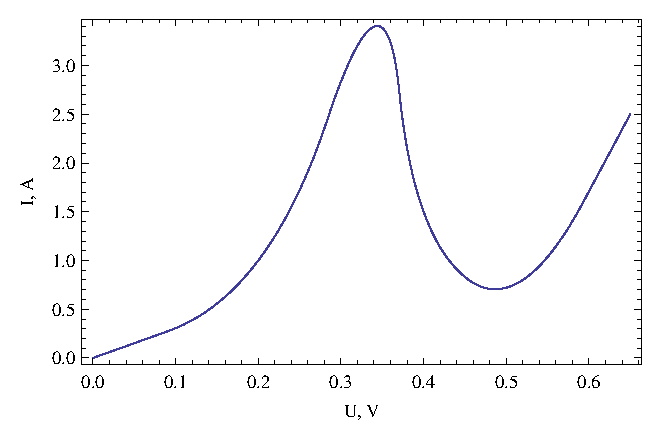
\includegraphics{bilder/resonante_tunneldiode_1.eps}
\end{figure}
\item Die Abbildung zeigt das U-I-Diagramm einer GaAs-RTD mit $l=5 \unit{nm}$. Für diese gilt $m^* = 0.067 m_e$. Wie breit ist das Energiespektrum des links eintreffenden Elektronenstromes?
\item Wie groß ist die Differenz zwischen den Energien der ersten beiden Niveaus? Reicht die thermische Energie bei Raumtemperatur um einen Großteil der Elektronen ins 2. Energieniveau zu bringen?
\end{abcenum}

\begin{solution}
\begin{abcenum}
\item $E_n = \frac{n^2 h^2}{8 l^2 m^*}$
\item Das Maximum ($U_1$) entspricht dem Punkt mit $\alpha e U_1 = E_1$, da danach ein steiler Abfall folgt, also ist $\alpha \approx 0.66$. Weiterhin ist die Breite des Energiespektrums $E_F = E_2 - E_1 - \alpha e (U_2 - U_1) \approx 0.55 \unit{eV}$, wobei $U_2$ das Minimum bezeichnet.
\item $E_2 - E_1 \approx 1\ee{-19}\unit{J}$, $\frac32 kT \approx 6\ee{-21}\unit{J}$, also reicht die thermische Energie dafür nicht aus.
\end{abcenum}
\end{solution}
\end{problem}


\begin{problem}{Lawine}{6}
\skizze{
\begin{pspicture}(-2.75,-0.5)(2.75,3.5)
\rput{30}(-2.5,0){
\pscircle(0,0.125){.125}
\pscircle(1,0.125){.125}
\pscircle(2,0.125){.125}
\pscircle(3,0.125){.125}
\pscircle(4,0.125){.125}
\pscircle(5,0.125){.125}
\pscircle(6,0.125){.125}
\psline(-0.25,0)(7,0)
\psline{<->}(4,-0.125)(5,-0.125)
\rput{-30}(4.5,-0.35){$d$}
\rput{-30}(5,0.55){$m$}
\rput{-30}(0,0){
\psline[linestyle=dashed](0,0)(2,0)
\psarc(0,0){0.5}{0}{30}
\rput(0.75,0.2){$\alpha$}
}
}
\psline{->}(2,1.5)(2,0)
\uput[r](2,0.75){$g$}
\end{pspicture}
}
Auf einem Hang, der den Winkel $\alpha$ mit der Horizonaten einschließt, liegen in konstanten Abständen $d$ identische Schneeflocken der Masse $m$. Die obere Flocke wird leicht angeschoben, sodass eine Lawine entsteht. Der Aufschlag der Lawine auf die ruhenden Flocken ist immer völlig inelastisch, die Gleitreibung kann vernachlässigt werden. Welche Beschleunigung hat die Lawine nachdem diese viele Flocken angesammelt hat?
\begin{solution}
Man betrachte die kontinuierliche Version des Problems und bezeichne die Position der Lawine auf dem Hang mit $l$, wobei $0$ der Lage der obersten Flocke entspricht und $l$ nach unten zunimmt. Die Bewegungsgleichung lautet dann
\[
l \ddot l + \dot l^2 = l g \sin\alpha.
\]
Mit dem Ansatz $l = \frac12 a t^2$ bekommt man
\[
a = \frac13 g \sin\alpha.
\]
\end{solution}
\end{problem}


\begin{problem}{Oberflaechentemperatur der Sonne}{3,5}
Man schätze die Temperatur der Sonnenoberfläche ausschließlich unter Verwendung der mittleren Erdoberflächentemperatur $T_E = 288 \unit{K}$ und des Winkeldurchmessers der Sonne bei der Betrachtung von der Erde aus $\phi = 32'$ ab.
\begin{solution}
\[
T_S = \frac{2 T_E}{\phi^{1/2}} \approx 5800 \unit{K}
\]
\end{solution}
\end{problem}


\begin{problem}{Wechselstromverbraucher}{6}
Es gibt mehrere einfache Schaltungen, die an das Stromnetz ($230 \unit{V}$, $50 \unit{Hz}$) angeschlossen eine elektrische Leistung von $400 \unit{W}$ umsetzen und dabei einen effektiven Strom von $8 \unit{A}$ durchlassen.
\begin{abcenum}
\item Man gebe alle möglichen Schlatungen dieser Art an, die aus minimal möglicher Anzahl von Elementen bestehen und gebe auch die entsprechenden Kennzahlen an.
\item Bei einer dieser Schaltungen eilt der Strom der Spannung voraus. Wenn man die Netzfrequenz verdoppelt, steigt der Phasenvorsprung um $8\%$. Um welche der Schaltungen handelt es sich dabei?
\end{abcenum}

\begin{solution}
\begin{abcenum}
\item Für den Gesamtwiderstand gilt
\[
|Z| = V_\mathrm{eff} / I_\mathrm{eff}
\]
\[
\Re Z = P / I_\mathrm{eff}^2
\]
Zu den 2 möglichen Impedanzen hat man jeweils eine Parallel- bzw. serielle Schaltung mit entweder Kondensator oder Spule und Widerstand.
\item $\Im Z < 0$ $\Rightarrow$ eine der Kondensatorschaltungen, wobei man leicht rausfinden kann, welche es ist.
\end{abcenum}
\end{solution}
\end{problem}


\begin{problem}{Mondabstandsmessung}{3,5}
Der Abstand zum Mond kann zentimetergenau mit einem Laserstrahl bestimmt werden, der an einem auf dem Mond aufgestellten Spiegel reflektieret wird. Eine der Fehlerquellen ist dabei die Atmosphäre, die einen von $1$ unterschiedlichen Brechungsindex besitzt und die Laufzeit damit verlängert. Wie groß ist die Auswirkung dieses Effekts auf das Messergebnis, wenn der Brechungsindex der Luft sich mit $n = 1 + \rho \eta$, $\eta = 0.00021 \unit{m^3/kg}$ ändert und der Luftdruck an der Oberfläche $p_0 = 101.3 \unit{kPa}$ beträgt?

\begin{solution}
Der Abstand scheint um
\[
\Delta l = \int_0^{+\infty} (n-1) \dif h = \int_0^{+\infty} \rho \eta \dif h = \frac{\eta}{g} \underbrace{\int_0^{+\infty} \rho g \dif h}_{=p_0} = \frac{p_0 \eta}{g}
\]
größer als in Wirklichkeit.
\end{solution}
\end{problem}


\begin{problem}{Kosmische Strahlung}{5,5}
Protonen können unter Abstrahlung eines Pions (Ruhemasse $135 \unit{MeV}$) an Photonen gestreut werden:
\[
p + \gamma \rightarrow p + \pi^0.
\]
Durch diesen Prozess wird die maximale Energie der Protonen kosmischer Strahlung begrenzt, da das Universum mit der Hintergrundstrahlung der Wellenlänge $1.9 \unit{mm}$ gefüllt ist. Wo liegt diese Obergrenze?

\begin{solution}
Die kleinste Energie wird benötigt wenn die entstehenden Teilchen nach dem Stoß zusammen weiterfliegen. Wenn $E$ die Energie des Protons, $E_p$ seine Ruheenergie und $p = \frac1c \sqrt{E^2 - E_p^2}$ sein Impuls bezeichnet, gilt dann
\[
(E+hf)^2 = (E_p + E_\pi)^2 + (p- h/\lambda)^2 c^2.
\]
Auflösen nach $E$ ergibt
\[
E = \frac{E_\pi (2 E_p + E_\pi)}{4 f h} + \frac{E_p^2 f h}{E_\pi (2 E_p +E_\pi)} \approx \frac{E_\pi (2 E_p + E_\pi)}{4 f h} \approx 1.2\ee{20} \unit{eV}.
\]
\end{solution}
\end{problem}


\begin{problem}{Membranenpotential}{5,5}
Eine Zellmembran lässt Kaliumkationen durch. Die Stromdichte hängt dabei vom Konzentrationsgradienten und vom elektrischen Feld ab:
\[
j = \mu E - D \tdif{c}{x}
\]
Die Dimension des Diffusionskoeffizienten ist dabei $\unit{m^2/s}$.
\begin{abcenum}
\item Leitfähigkeitskoeffizient $\mu$ hängt im Wesentlichen vom Diffusionskoeffizienten, der Ladung der einzelnen Ionen, ihrer Konzentration, der Temperatur und der Boltzmannkonstante ab. Man leite mittels einer Dimensionsanalyse diesen Zusammenhang her. Die auftretenden numerischen Koeffizienten sind zu vernachlässigen.
\item Was ist dann die Gesamtstromdichte?
\item Wie groß ist die Spannung an der Zellmembrag in einem Gleichgewichtszustand wenn die Kaliumkationenkonzentration im Inneren der Zelle $135 \unit{mol/m^3}$ und außerhalb der Zelle $5 \unit{mol/m^3}$ beträgt, die Membran für keine anderen Ionen durchlässig ist und die Umgebungstemperatur $300 \unit{K}$ beträgt?
\end{abcenum}

\begin{solution}
\begin{abcenum}
\item $\mu \sim \frac{cDq_e}{kT}$
\item $j = D \left( \frac{cq}{kT} \tdif{\phi}{x} - \tdif{c}{x} \right)$
\item $j=0$, $\frac{cq}{kT} \tdif{\phi}{x} = \tdif{c}{x}$
\[
\frac{q}{kT} \dif\phi = \frac{\dif c}{c} \quad | \int
\]
\[
\Delta \phi = \frac{kT}{q_e} \ln \frac{c_\mathrm{innen}}{c_\mathrm{außen}} \approx 0.085 \unit{V}
\]
\end{abcenum}
\end{solution}
\end{problem}


\begin{problem}{Huepfender Ball}{7}
Ein Ball fällt ohne zu rotieren mit einer Geschwindigkeit $v=10 \unit{m/s}$ unter einem Winkel $\alpha = \frac\pi4$ auf den Boden. Wie weit wird er nach dem Stoß fliegen, wenn der Gleitreibungskoefizient zwischen Ball und Boden $\mu = 0.1$ beträgt? Wie ändert sich dieses Ergebnis, wenn $\mu = 0.8$ ist?\\
\hinweis Der Ball kann als dünne Kugelschale (Trägheitsmoment um eine Schwerpunktachse $\frac23 m r^2$), der Stoß als kurz und die Luftreibung als unwesentlich angesehen werden.
\begin{solution}
Für den übertragenen Impuls in horizontale Richtung gilt
\[
\frac{\Delta p_h}{m} \leq \frac{\Delta p_v}{m}, \quad \frac{\Delta p_h}{m} \leq \frac23 \omega R
\]
In den beiden Fällen tritt bei einer der Ungleichungen Gleichheit ein. Wenn man nun noch Energie- und Impulserhaltung verwendet, bekommt man genügend Gleichungen um die Geschwindigkeit des Balls und ihre Richtung nach dem Stoß zu berechnen. Man bekommt schließlich\\
$\mu = 0.1$ $\Rightarrow$ $l \approx 8.2 \unit{m},$\\
$\mu = 0.8$ $\Rightarrow$ $l \approx 6.1 \unit{m}.$
\end{solution}
\end{problem}











%\newpage
%\subsection*{2009 -- 3. Runde -- Theoretische Klausur I}

\begin{problem}{Linse vor dem Spiegel}{4}
Eine dünne Linse erzeugt ein Bild eines Objektes. Direkt hinter die Linse wird nun parallel zur selben ein flacher Spiegel gestellt. Die Größe, wenn nicht die Lage, des Bildes bleibt unverändert. Man bestimme die Vergrößerung.
%\begin{solution}
%\end{solution}
\end{problem}

\begin{problem}{Kondensatoren und Dioden}{5}
\skizze{
\psset{unit=0.75cm}
\begin{pspicture}(-2,-1)(6,4)
\pnode(0,0){Erde1}
\pnode(2,0){Erde2}
\pnode(4,0){Erde3}
\pnode(0,3){U1}
\pnode(2,3){A}
\pnode(4,3){B}

\tension[labeloffset=1](Erde1)(U1){$U(t)$}
\capacitor[labeloffset=-1](U1)(A){$C$}
\capacitor[labeloffset=-1](Erde3)(B){$2 C$}
\diode(B)(A){}
\diode(A)(Erde2){}
\ground(Erde2)
\wire(Erde1)(Erde2)
\wire(Erde2)(Erde3)
\nput{90}{A}{$A$}
\nput{90}{B}{$B$}
\end{pspicture}
}
An der dargestellten Schaltung wird eine Rechteckspannung $U(t)$ mit Grenzwerten $\pm U_0$ und Pulsdauer $\tau$ angelegt. Man bestimme das asymptotische Verhalten der Potentiale in der Punkten $A$, $B$ unter der Annahme dass die Kondensatoren und die Dioden ideal sind.
%\begin{solution}
%\end{solution}
\end{problem}

\begin{problem}{Erwärmung durch Strahlung}{3,5}
Im Mittelpunkt eines wassergefüllten perfekt isolierten kugelförmigen Gefäßes befindet sich eine Probe eines radioaktiven Isotops, bei dessen Zerfall ein Elektron und ein Photon freigesetzt werden. Die Elektronen werden vom Wasser weitgehend komplett absorbiert, die Photonen nicht. Wie lange dauert es bis das Wasser anfängt zu sieden? Man nehme an, die Temperatur sei in dem Gefäß stets überall gleich, Druckausgleich zur Atmosphäre gegeben und das Volumen der Probe vernachlässigbar.
\begin{center}
\begin{tabular}{lc}
\toprule
Radius des Gefäßes & $r = 10 \unit{cm}$\\
Stoffmenge der Probe & $n = 5 \unit{mol}$\\
Halbwertszeit des Isotops & $T_{\frac12} = 5 \unit{a}$\\
Energie der freigesetzten Elektronen & $E_\beta = 310 \unit{keV}$\\
Energie der freigesetzten Photonen & $E_\gamma = 1200 \unit{keV}$\\
Halbwertschicht der Photonen der Energie $E_\gamma$ in Wasser & $d_{\frac12} = 15 \unit{cm}$\\
Spezifische Wärmekapazität von Wasser & $c = 4.19 \unit{kJ \cdot kg \cdot K^{-1}}$\\
Dichte von Wasser & $\rho = 1000 \unit{kg \cdot m^{-3}}$
\bottomrule
\end{tabular}
\end{center}
%\begin{solution}
%\end{solution}
\end{problem}


\begin{problem}{Die Stumme von Koeln}{5,5}
Die 1878 aufgehängte Kaiserglocke des Kölner Doms war von zahlreichen technischen Problemen geplagt. Zunächst schien die falsche Tonlage das größte darzustellen, doch hat man nach dem Einbau gemerkt dass man nicht mal den falschen Ton erzeugen konnte, da sich der Klöppel beim Schwingen relativ zur Glocke kaum bewegte, was den Kölnern natürlich auch den misslichen Klang ersparte.\\
Unter welchen Bedingungen an relevante Parameter bleibt der Klöppel bei kleinen Schwingungen relativ zur Glocke in Ruhe? Dieser ist innerhalb der Glocke auf der Symmetrieachse im Abstand $l$ vom Aufhängepunkt der Glocke aufgehängt. Die jeweiligen Massen $m_g$, $m_k$, Schwerpunktabstände zu den Aufhängepunkten $s_g$, $s_k$ sowie reduzierte Pendellängen $l_g$, $l_k$ der Glocke bzw. des Klöppels sind bekannt. \hinweis Die reduzierte Pendellänge ist die Länge eines idealisierten Pendels der die gleiche Schwingungsdauer besitzt wie das betrachtete Pendel. Die Masse des Klöppels ist klein verglichen  mit der Masse der Glocke.
%Wie groß muss demnach $l$ gewesen sein?
%%%% Hier wären noch Zahlenangaben %%%%%%
\begin{solution}
Wenn die beiden Pendel mit gleicher Frequenz schwingen schwingen sie praktisch unabhängig voneinander. Da die Schwingungsdauer die Pendellänge eindeutig bestimmt muss $l_g = l + l_k$ gelten.
\end{solution}
\end{problem}

\begin{problem}{Flasche mit Unterdruck}{6}
In einer Flasche befindet sich anfangs Luft bei Außentemperatur $T_0$ und halbem Außendruck $p_0$. Die Flasche wird kurz geöffnet sodass ein Druckausgleich stattfindet und gleich wieder verschlossen.
\begin{abcenum}
\item Welche Temperatur hat die Luft in der Flasche gleich danach?
\item Welcher Druck stellt sich in der Flasche nach einiger Zeit ein?
\end{abcenum}
\begin{solution}
Man bezeichne die Anzahl der Moleküle in der Flasche mit $N$, den Druck mit $p$, das Volumen mit $V$, die Energie mit $E$, die Temperatur mit $T$, die Zahl der Freiheitsgrade pro Molekül mit $\phi$. Dann gilt am Anfang
\[
N = \frac{p_0 V}{2 k T_0}, \quad p = \frac{p_0}{2}, \quad E = \frac{\phi}{2} N k T_0.
\]
Die Energieänderung bei Einströmen von $\dif N$ Molekülen ist
\[
\dif E = \underbrace{\frac\phi2 \dif N k T_0}_\mathrm{Waerme} + \underbrace{p_0 \frac{\dif N k T_0}{p_0}}_\mathrm{Mechanische Arbeit} = \frac{\phi+2}{2} k T_0 \dif N.
\]
Es gilt stets
\[
T=\frac{2 E}{\phi}\frac{1}{N k}, \quad  p = \frac{NkT}{V} = \frac{2 E}{\phi} \frac1V = \frac{2}{\phi V}  E
\]
Wenn man nun mit 0 den Anfangszustand, mit 1 den Zustand gleich nach dem Druckausgleich und mit 2 den Zustand nach dem Erreichen des thermischen Gleichgewichts bezeichnet, bekommt man
\[
N(2) = N(1) = N(0) + \frac{E(1) - E(0)}{\frac{\phi+2}{2} k T_0} = \frac{p_0 V}{2 k T_0} + \frac{p_0 V \frac{\phi}{2} - p_0 V \frac{\phi}{4}}{\frac{\phi+2}{2} k T_0} = \frac{p_0 V}{k T_0} \left( \frac12 + \frac1{2\gamma} \right)
\]
\[
T(1) = \frac{2 E(1)}{\phi}\frac{1}{N(1) k} = \frac{V p(1)}{N(1) k} = \frac{V p_0}{N(1) k} = \frac{2 T_0}{1+1/\gamma}
\]
\[
p(2) = \frac{N(2) k T(2)}{V} = \frac{p_0 V}{k T_0} \left( \frac12 + \frac1{2\gamma} \right) \frac{k T_0}{V} = p_0 \left( \frac12 + \frac1{2\gamma} \right)
\]
\end{solution}
\end{problem}

\begin{problem}{Verstopfter Abfluss}{6}
Eine Badewanne hat einen kreisförmigen Abfluss (Radius $r = 2\unit{cm}$), den ein Korrektor mangels eines Stöpsels mit einem Ball (Radius $r = 5\unit{cm}$, Dichte $\rho$) zu verschließen versucht. Dies gelingt ihm anfangs nicht, weil der Ball bei einer bestimmten Wasser-(Dichte $\rho_W = 1000 \unit{kg \cdot m^{-3}}$)-höhe $h$ aufzusteigen beginnt. Nachdem der Badende resigniert beschließt den Ball die ganze Zeit über zu halten und die Badewanne füllt, stellt er verwundert fest, dass der Ball ab eier Wasserhöhe von $H = 15 \unit{cm}$ ohne zusätzlichen Halt am Platz bleibt.
\begin{abcenum}
\item Wie groß ist die Dichte des Balls?
\item Ab welchem Füllstand $h$ muss man ihn vorübergehend halten?
\end{abcenum}
\hinweis Das Volumen einer Kugelkappe mit Krümmungsradius $R$ und Schnittflächenradius $r$ beträgt $\frac\pi3 \left( 2 R^3 - (2 R^2 + r^2) \sqrt{R^2 - r^2} \right)$.
\begin{solution}
Bei vollständiger Bedeckung wirkt auf den Ball außer seiner eigenen Gewichtskraft
\[
F_g = \frac43 \pi g \rho R^3
\]
die Gewichtskraft der Wassersäule direkt über dem Abfluss
\[
F_s = g \left( \pi r^2  \left( H - 2 \sqrt{ R^2  - r^2 } \right) - \frac\pi3 \left( {2 {R}^{3} } - \left( {2 {R}^{2} } + {r}^{2}  \right) {\sqrt{ {R}^{2}  - {r}^{2}  } } \right) \right) \rho_{W}
\]
sowie die Auftriebskraft des Teils des Balls der sich nicht direkt über dem Abfluss befindet
\[
F_a = {g \left( \frac43 \pi R^3 - 2 \frac\pi3 \left( {2 {R}^{3} } - \left( {2 {R}^{2} } + {r}^{2}  \right) {\sqrt{ {R}^{2}  - {r}^{2}  } } \right) - {{{2 \pi} {r}^{2} } \sqrt{ {R}^{2}  - {r}^{2}  }} \right)} \rho_{W}
\]
Aus dem Kräftegleichgewicht $F_g + F_s = F_a$ ergibt sich die Dichte des Balls zu
\[
\rho  =  \frac{\rho_{W}}{4 R^3 } \left( 2 R^3  + \sqrt{ R^2  - r^2  } \left( {2 {R}^{2} } + {r}^{2}  \right) - 3 H r^2 \right).
\]
Bei geringen Füllhöhen hat man für den Schnittflächenradius der Kugel an der Wasseroberfläche
\[
r_s = \sqrt{ {R}^{2}  - {\left( \sqrt{ {R}^{2}  - {r}^{2}  } - h \right)}^{2}} \approx \frac{{h \sqrt{ {R}^{2}  - {r}^{2}  }}}{r} + r
\]
und für die Auftriebskraft damit (in quadratischer Näherung)
\[
F_{ak} \approx \frac{\pi g h^2}{2 r^2 \sqrt{R^2 - r^2}} \left( 3 R^2 r^2 - 2 r^4 \right) \rho_{W}
\]
was mit $F_{ak} = F_g$ auf folgendes Ergebnis führt:
\[
h  =  2 R  \sqrt{ \frac{2 R \sqrt{R^2 - r^2} \rho}{3( 3 R^2 - 2 r^2 ) \rho_W } 
\]
\end{solution}
\end{problem}









%\newpage
%\subsection*{2009 -- 3. Runde -- Theoretische Klausur II}

\begin{problem}{Federn am Haken}{3,5}
Es werden $n$ identische Punktmassen $m$ durch ideale Federn der Ruhelänge $l$ und Federkonstanten $k_1,\dots, k_n$ in eine Kette verbunden sodass die erste Feder noch an einem Haken befestigt ist. Wenn die Kette im Weltall mit Winkelgeschwindigkeit $\omega$ um den Haken rotiert haben alle Federn wieder die gleiche Länge $L$. Man bestimme alle Federkonstanten.
\begin{solution}
Die Spannung der $i$-ten Feder ist
\[
(L-l) k_i = \sum_{j=i}^n m \omega^2 (jL).
\]
Damit bekommt man für die Federkonstanten
\[
k_i = \frac{m \omega^2 L}{2 (L-l)} \left( n(n+1) - i(i-1) \right)
\]
\end{solution}
\end{problem}

\begin{problem}{Logarithmisches Potentiometer}{4,5}
Für eine Gravizapa braucht man ein Potentiometer, bei dem sich der Widerstand logarithmisch mit dem Abgriff ändert: $R(x) = R_0 \ln(1+x/k)$, wobei $R_0 = 1 \unit{\Omega}$. Diese werden üblicherweise von Pazaken aus Metallstreifen mit dem spezifischen Widerstand $\rho = 1.5\ee{-6} \unit{\Omega\cdot m}$, Länge $a = 1\unit{m}$ und Breite $b = 1\unit{mm}$ geschliffen.
\begin{abcenum}
\item Wie muss das Dickeprofil des fertigen Potentiomenters $h(x)$ beschaffen sein wenn man $k=a$ voraussetzt?
\item (Bonusfrage) Wie viel KC kostet eine Gravizapa? Es muss nämlich $k=1000 a$ gelten. Wie genau muss ein Pazak arbeiten um das entsprechende Potentiometer herstellen zu können? Zur Auswahl stehende Herstellungsmethoden: Gießen, Fräsen, Ätzen, Lithographie, Maxwelldämon.
\end{abcenum}
%\begin{solution}
%\end{solution}
\end{problem}


\begin{problem}{Teilchendetektion}{4,5}
In einem Teilchenbeschleuniger wird ein kurzlebiges Teilchen erzeugt das fast sofort in zwei andere zerfällt. Diese werden von Detektoren aufgefangen und als Elektron bzw. Positron identifiziert. Deren Impulse werden dabei registriert, die Ergebnisse sind hier komponentenweise angegeben:
\begin{center}
\begin{tabular}{lccc}
\toprule
Teilchen & $c \cdot p_x, \unit{GeV}$ & $c \cdot p_y, \unit{GeV}$ & $c \cdot p_z, \unit{GeV}$ \\
\midrule
Elektron & -12 & 49 & -50 \\
Positron & 21 & -32 & -31 \\
\bottomrule
\end{tabular}
\end{center}
Welchen Impuls, Energie und Ruheenergie besaß das zerfallene Teilchen? Welches der aufgeführten Teilchen könnte es gewesen sein?
\begin{center}
\begin{tabular}{lccc}
\toprule
Teilchen & Ruheenergie, $\unit{MeV}$ & Ladung & Spin \\
\midrule
Elektron & 0.51 & -1 & 1/2 \\
Positron & 0.51 & +1 & 1/2 \\
Proton & 940 & +1 & 1/2 \\
Up-Quark & 2 & +2/3 & 1/2 \\
Myon & 105 & -1 & 1/2 \\
$W^+$ & 80400 & +1 & 1 \\
$W^-$ & 80400 & -1 & 1 \\
$Z_0$ & 91100 & 0 & 1 \\
Photon & 0 & 0 & 1 \\
\bottomrule
\end{tabular}
\end{center}
\begin{solution}
Der Impuls des Teilchens betrug
\[
\vec p = \vec p_\mathrm{Elektron} + \vec p_\mathrm{Positron} = (9,\, 17,\, -81)^T \unit{GeV}/c.
\]
Die Ruheenergie des Elektrons bzw. des Positrons kann vernachlässigt werden. Die Energie des Teilchens betrug also etwa
\[
E \approx (|\vec p_\mathrm{Elektron}| + |\vec p_\mathrm{Positron}|) c \approx 120 \unit{GeV}.
\]
Für die Ruhemasse bekommt man
\[
m^2 c^2 \approx 2 |\vec p_\mathrm{Elektron}|  |\vec p_\mathrm{Positron}| - 2 \vec p_\mathrm{Elektron} \cdot \vec p_\mathrm{Positron}, \quad m \approx 87 \unit{GeV} / c^2
\]
Von der Masse her kommen also $W^+$, $W^-$ und $Z_0$ in Frage. Da die elektrische Ladung erhalten ist muss es also $Z_0$ sein.
\end{solution}
\end{problem}


\begin{problem}{Fata Morgana}{5}
Eine Wüste, aber auch eine lange gerade Straße erscheint bei extremer Hitze oft nass. Dies liegt an der heißen Luftschicht direkt über dem Boden, die flach einfallendes Licht z.B. von Himmel reflektiert. Wie heiß muss die Luft direkt an der Oberfläche sein damit man bei einer Augenhöhe von $H = 1.5 \unit{m}$ in einer Entfernung von $L = 200 \unit{m}$ den Anfang der Spiegelung beobachtet? Man gehe davon aus dass die Temperatur der Luft nur von der Höhe abhängt. Der Brechungsindex hängt mit der Luftdichte über $n-1 \sim \rho$ zusammen. Die Temperatur der Luft auf Augenhöhe beträgt $T_0 = 20 \cel$, die Dichte $\rho_0 = 1.204 \unit{kg \cdot m^{-3}}$, Brechungsindex $n_0 = 1 + n_\Delta$, $n_\Delta = 2.92\ee{-4}$. \hinweis Die Druckänderung über die betrachtete Höhe kann vernachlässigt werden, der Druck ist also konstant $p = 1 \unit{atm}$.
\begin{solution}
Man betrachte einen Lichtstrahl, der vom Betrachter ausgeht und scheinbar in Entfernung $L$ endet. Für den Winkel den dieser mit der Vertikalen einschließt gilt
\[
\tan\alpha = \frac{L}{H}, \quad \sin\alpha = \frac{L}{\sqrt{L^2 + H^2}}
\]
Da die Isothermen parallel zum Boden verlaufen, kann das Brechungsgesetz verwendet werden. Die Bedingung dass der Strahl am Boden gerade noch umkehrt lässt sich schreiben als
\[
n_0 \sin\alpha = n_\mathrm{Boden} \sin\frac\pi2 = n_\mathrm{Boden}.
\]
Da die Luftdichte bei konstantem Druck umgekehrt proportional zur Temperatur ist, gilt
\[
n_\mathrm{Boden} = 1 + n_\Delta \frac{\rho_\mathrm{Boden}}{\rho_0} = 1 + n_\Delta \frac{T_0}{T_\mathrm{Boden}}
\]
und damit
\[
T_\mathrm{Boden} = \frac{ n_\Delta T_0 }{ n_0 \sin\alpha - 1 }
\]
\end{solution}
\end{problem}


\begin{problem}{Feder als Spule}{5}
Durch eine spiralförmige Feder mit Radius $r = 5 \unit{cm}$, Federkonstante $k = 1 \unit{N/m}$) und $N = 400$ Windungen fließt ein Strom $I = 1 \unit{A}$. Die Länge der Feder beträgt dabei $L = 40 \unit{cm}$. Wie groß ist die Ruhelänge $l$ der Feder?
\begin{solution}
Die Magnetische Feldstärke innerhalb der Spule ist in erster Näherung konstant
\[
B = \frac{\mu_0 I N}{L}.
\]
Die Energie des Magnetfeldes ist
\[
E_f = \int \frac{B^2}{2 \mu_0} \dif V = \frac{\pi r^2 \mu_0 I^2 N^2 }{2 L}
\]
und die Spannenergie der Feder
\[
E_s = \frac12 k \left( L - l \right)^2.
\]
Da in diesem Fall die Lagrangefunktion $\mathcal L =E_f - E_s + \frac12 m_\mathrm{eff} \dot L^2$ lautet, ist die Gleichgewichtsbedingung
\[
0 = \ddot L \sim \tdif{}{t} \pdif{}{\dot L} \mathcal L = \pdif{}{L} \mathcal L =  - \frac{\pi r^2 \mu_0 I^2 N^2 }{2 L^2} - k \left( L - l \right),
\]
was auf die Ruhelänge
\[
l  =  L + \frac{\pi r^2 \mu_0 I^2 N^2 }{2 k L^2}
\]
führt.
\end{solution}
\end{problem}


\begin{problem}{Wasserrakete}{7,5}
Eine Flasche (Volumen $V_g = 2  \unit{l}$, Masse $M = 200 \unit{g}$) wird zur Hälfte mit Wasser gefüllt. Der restliche Teil enthält komprimierte Luft. Die Flasche wird mit dem Verschluss (Radius $r = 1 \unit{cm}$) nach unten auf Meereshöhe aufgestellt. Dieser wird anschließend geöffnet.
\begin{abcenum}
\item Wie groß muss der Druck in der Flasche sein damit diese abhebt?
\item Wie groß muss der Druck sein damit die Flasche weiter beschleunigt bis das Wasser ausgeht?
\end{abcenum}
Die Reibung kann vernachlässigt werden. Weiterhin ist der Durchmesser der Flasche als groß gegenüber dem des Verschlusses anzunehmen. Diese Aufgabe zeigt übrigens eindrucksvoll warum ein Pepelaz ohne Gravizapa nutzlos ist.
%\begin{solution}
%\end{solution}
\end{problem}

\Closesolutionfile{solutions}
\setcounter{numlabel}{0}
\Opensolutionfile{expsolutions}[AUTO_LOESUNGSDATEI_EXP]



\section*{Experimentelle Aufgaben}

Bei den experimentellen Aufgaben ist generell davon auszugehen, dass Millimeterpapier und Zeichengerät gegeben sind. Wenn es um Stromkreise geht, stehen immer ausreichend viele Kabel, Krokodilklemmen, etc. zu Verfügung.\\
Die Zeichnungen der Blackboxen werden in den Klausuren selbstverständlich nicht angegeben.

\begin{problem}{Ein Rollpendel}{22}
In einer ca. $8\unit{cm}$ großen runden Blechdose ist an einer Seite der Innenwand ein Zusatzgewicht angebracht. Der Schwerpunkt ist somit seitlich verschoben.\\
\\
Materialien:
\begin{itemize}
\item exzentrische Dose
\item Stativstange
\item Stoppuhr
\item Schere
\item Bindfaden
\item Lineal (kann auch als Experimentiergerät dienen)
\item Gewicht $46\unit{g}$
\end{itemize}
Aufgaben:
\begin{abcenum}
\item Bestimmen Sie mit Hilfe von Rollschwingungen das Trägheitsmoment $J$ der exzentrischen Dose bezüglich ihrer Zylinderachse. (Tipp: Energieansatz)\\
Dazu benötigen Sie die Ergebnisse der Teilaufgaben 2. und 3. \emph{(11 Punkte)}
\item Bestimmen Sie den Abstand $s$ des Schwerpunktes der Dose von ihrer Mittelachse. \emph{(7 Punkte)}
\item Bestimmen Sie die Masse $M$ der Dose. \emph{(4 Punkte)}
\end{abcenum}
\hinweis
\begin{itemize}
\item Für kleine Winkel gelten die Näherungen $\sin{\varphi}\approx\varphi$ und $\cos{\varphi}\approx1-\frac{\varphi^2}{2}$.
\item Der steinersche Satz besagt für das Trägheitsmoment eines Körpers um eine um $a$ vom Schwerpunkt entfernte Achse
\[
J=J_s+M\cdot a^2,
\]
wobei $J_s$ das Trägheitmoment bezüglich einer parallel verlaufenden Schwerpunktachse bezeichnet.
\end{itemize}
\begin{expsolution}
\begin{abcenum}
\item Rollschwingungen mit Schwingungsgleichungen
\item Die Dose am Faden pendeln lassen. Einmal mit Schwerunkt oben, einmal unten.
\[
\Rightarrow\qquad s=\frac{\Delta T}{2\pi}\sqrt{g\left(\Delta T^2g-4l\right)}\quad?
\]
\item Das Lineal im Schwerpunkt aufhängen und als Balkenwaage für Festgewicht und Dose verwenden.
\end{abcenum}
\end{expsolution}
\end{problem}

\begin{problem}{Gleichstromblackbox mit 3 Anschluessen}{10}
\skizze{
\psset{unit=0.68cm}
\begin{pspicture}(-4,-1)(4,4)
\pnode(-2,0){A}
\pnode(2,0){B}
\pnode(0,3){C}
\resistor(A)(C){}
\resistor(B)(C){}
\lamp(A)(B){}
\end{pspicture}
}
Materialien:
\begin{itemize}
\item Gleichstrom Blackbox mit 3 Anschlüssen
\item Gleichstrom Netzgerät $0-7,5\unit{V}$
\item 2 Digitalmultimeter
\end{itemize}
In der Blackbox befindet sich zwischen je 2 Anschlüssen genau eine der folgenden 3 Möglichkeiten:\\ Nichts, ein ohmscher Widerstand (insgesammt nur eine Sorte) oder ein Glühlämpchen (nur eine Sorte).
\begin{abcenum}
\item Welche Elemente befinden sich in der Blackbox und wo?
\item Wie groß sind ggf. die Festwiderstände und wie groß ist ggf. die Leistung der Glühbirne bei $7,5\unit{V}$?
\end{abcenum}
\hinweis bei zu hohen Spannungen können die Elemente der Blackbox beschädigt werden!
\begin{expsolution}
Widerstände grob messen (Symmetrie?) $\rightarrow$ einzelne Verbindungen kurzschließen $\rightarrow$ Elemente genau vermessen $\rightarrow$ Zwei Widerstände und ein Lämpchen
\end{expsolution}
\end{problem}

\begin{problem}{Verlustleistung eines Kondensators}{10}
Materialien:
\begin{itemize}
\item Kondensator
\item Widerstand $1\unit{k\Omega}$
\item Wechselstrom Netzgerät $8\unit{V},\; 50\unit{Hz}$
\item 2 Digitalmultimeter
\end{itemize}
Aufgaben:
\begin{abcenum}
\item Welche Kapazität besitzt der Kondensator unter der Annahme, dass es sich um einen idealen Kondensator handelt?
\item Der reale Kondensator besitzt auch einen ohmschen Widerstand. Wie groß ist dieser? Wie groß ist dann die wirkliche Kapazität? Verwenden Sie dazu geeignete Schaltungen und geben diese an! Vergleichen Sie das Ergebnis mit dem aus (a)!
\end{abcenum}
\begin{expsolution}
\begin{abcenum}
\item $C_i=\frac{1}{Z\cdot 2\pi f}$
\item Mit Volt- und Amperemeter misst man den Scheinwiderstand.\\
Beim Kondensator: $Z^2=R_C^2+(\frac{1}{\omega C})^2$.\\
Mit Widerstand in Reihe: $Z_1^2=(R+R_C)^2+(\frac{1}{\omega C})^2$
\[
\Rightarrow\quad R_C=\frac{Z_1^2-Z^2-R^2}{2R}
\]
\[
C=\frac{R}{\pi f \sqrt{2(R^2Z^2+R^2Z_1^2+Z^2Z_1^2)-(R^4+Z^4+Z_1^4)}}
\]
Die Formel für $C$ sieht sehr kompliziert aus, besitzt aber hohe Symmetrie. Die Formel für den rein kapazitiven Widerstand entspräche der Formel für die Höhe in einem Dreieck.
\end{abcenum}
\end{expsolution}
\end{problem}



\begin{problem}{Coladose}{20}
Materialien:
\begin{itemize}
\item 1 Coladose, die in Wasser gerade noch schwimmt
\item Stoppuhr
\item großer Standzylinder, etwa $1\unit{m}$ hoch
\item Messbecher
\item 2 Messzylinder (50 bzw. 250 ml)
\item Wasser ($\rho = 1000 \unit{kg \cdot m^{-3}}$, wer hätte es gedacht)
\item Knete
\item Tücher zum Abtrocknen
\end{itemize}

\begin{abcenum}
\item Man bestimme $g$ mithilfe von Coladose, Lineal und Stoppuhr. Man beachte, dass die Coladose im Aufbau unbedingt sinnvoll zu verwenden ist!
\item Man lasse nun die Coladose vorsichtig in den Standzylinder gleiten, sodass die obere Fläche trocken bleibt. Wenn man die Dose leicht auslenkt, schiwngt diese eine Weile, kommt aber schnell zu Ruhe. Dies liegt an der Reibung, die sich in diesem Fall folgendermaßer beschreiben lässt:
\[
\vec{F}=-b \vec{v}
\]
Man bestimme $b$ auf 2 verschiedene Weisen: indem man eine Schwingung betrachtet und indem man die Dose unter Wasser hält, loslässt und den Aufstiegsvorgang beobachtet.
\item Nun darf die Dose geöffnet werden. Allerdings ist es nicht ratsam, alles gleich auszutrinken, denn nun geht es darum, die Dichte von Cola sowie die Masse der leeren Dose zu bestimmen. Viel Spaß!
\end{abcenum}

% \begin{expsolution}
% 
% \end{expsolution}
\end{problem}



\begin{problem}{Graphit}{6}
Bestimmen Sie mit den angegebenen Materialien möglichst genau den spezifischen Widerstand von Graphit. \hinweis Die Messung des Radiuses des Graphitstabes mit dem Lineal ist sehr ungenau.
\begin{itemize}
\item Graphitmine
\item Lineal
\item 2 Multimeter
\item 1 Batterie mit eingebautem Vorwiderstand
\item Objektträger
\end{itemize}
% \begin{expsolution}
% 
% \end{expsolution}
\end{problem}



\begin{problem}{Kupfer unnd Messing}{14}
Materialien:
\begin{itemize}
\item Eine Kupfer- und eine Messingplatte gleicher Größe und Dicke
\item 1 Stabmagnet
\item Stativmaterial
\item Stoppuhr
\item Fäden
\item Textilklebeband, Knete
\item Karton
\end{itemize}
Kupfer hat einen spezifischen Widerstand von $1.77 \ee{-8} \unit{\Omega m}$. Man bestimme den spezifischen Widerstand von Messing.
% \begin{expsolution}
% 
% \end{expsolution}
\end{problem}



\begin{problem}{Optische Blackbox}{20}
\skizze{
\psset{unit=0.55cm}
\begin{pspicture}(0,-0.5)(10,4.5)
\psline(0,0)(10,0)
\psline{-|}(0,4)(8,4)
\psline{|-}(9,4)(10,4)
\psline[linestyle=dotted](0,0)(0,4)
\psline[linestyle=dotted](10,0)(10,4)
\psarc(3,2){4.47}{333.5}{26.5}
\psarc(11,2){4.47}{153.5}{206.5}
\end{pspicture}
}
Materialien:
\begin{itemize}
\item 1 Blackbox
\item 1 Lichtquelle
\item 1 Meterstab
\item 1 Schirm
\item Wasser (Brechunsgindex $1.33$)
\end{itemize}
\begin{abcenum}
\item Die Blackbox besteht aus einem schwarzen Rohr, im Inneren dessen eine Linse befestigt ist. Beide Enden des Rohres sind mit Glasplatten verschlossen. Man bestimme mit zwei unterschiedlichen optischen Methoden die Brennweite und die Lage der Linse in der Blackbox.
\item An einer Seite der Linse besitzt die Blackbox eine Öffnung, durch die sich eine Hälfte der Blackbox mit Wasser füllen lässt, sodass Wasser nicht an die andere Seite der Linse kommt. Man bestimme die Krümmung der Linse und den Brechungsindex des Linsenmaterials.
\end{abcenum}

\begin{expsolution}
\begin{abcenum}
 \item \textbf{Methode 1:} Die Linse wird ein Stück von der Lampe aufgestellt. Dann wird der Schirm so positioniert, dass eine scharfe Abbildung des Glühwendels enteteht. Nun dreht man die Blackbox um und verschiebt sie so weit, bis die Abbildung wieder scharf ist. Aus der Verschiebung ergibt sich die Linsenposition. Kennt man diese, ergibt sich die Brennweite aus der Abbildungsgleichung $\frac 1 f = \frac 1 b + \frac 1 g$.\\
 \textbf{Methode 2:} Es wird eine scharfe Abbildung des Glühwendels erzeugt. daraufhin verschiebt man die Lampe seitlich. Auch das Bild verschiebt sich seitlich. Der Strahlensatz liefert nun die Position. Die Brennweite ergibt sich wie im ersten Fall.\\
 \textbf{Methode 3:} Man misst die Größe der scharfen Abbildung in Abhängigkeit vom Schirmabstand. Ein geeigneter Graph der Werte zeigt dann die Linsenposition. Die Brennweite ergibt sich wie im ersten Fall.
 \item Die Linsenmacherformel lautet in diesem Fall:
\[
 \frac r f = 2n-(1+1.33)
\]
Die Messung mit und ohne Wasser liefert mit den Daten aus a) zwei verschiedene Gleichungen, die man lösen kann. Unter der Annahme achsennaher Strahlen bewirkt die Brechung an der wassergefüllten Seite eine Verkürzung des Strahlenganges in der Luft um den Faktor $1.33$. Das muss man noch in die Rechnung mit einbeziehen.
\end{abcenum}
\end{expsolution}
\end{problem}



\begin{problem}{Unbekannte Spannungsquelle}{8}
Materialien:
\begin{itemize}
\item Eine Blackbox mit 2 Anschlüssen
\item 1 Amperemeter
\item 1 Widerstand von $620 \unit{k\Omega}$
\item 1 Kondensator
\item 1 Stoppuhr
\end{itemize}
In der Blackbox  mit 2 Anschlüssen befindet sich eine Gleichspannungsquelle. Bestimmen sie die Spannung dieser Spannungsquelle sowie die Kapazität des gegebenen Kondensators.
\begin{expsolution}
Bestimmung der Spannung: Reihenschaltung mit dem Widerstand:
\[
U = R\cdot I
\]
Bestimmung der Kapazität: Laden des Kondensators, dann Zeit stoppen, umpolen und über den Widerstand entladen:
\[
I(t) = I_0\cdot e^{-\frac{t}{R\,C}}
\]
In kurzen Zeitintervallen (z.B. 4s) die Wertepaare $(I|t)$ notieren. Im Diagramm $t(\ln I)$ auftragen und die Steigung $m$ ablesen.
\[
C = -\frac m R \qquad\qquad C \approx 10\unit{\mu F}
\]
\end{expsolution}
\end{problem}



\begin{problem}{Widerstaende und Dioden}{12}
\skizze{
\psset{unit=0.75cm}
\begin{pspicture}(-1,-1)(7,5)
\pnode(0,4){A}
\pnode(3,0){B}
\pnode(6,4){C}
\pnode(3,4){M}
\pnode(3,2){N}
\pnode(3,1){N2}
%Widerstände
\resistor(A)(M){}
\resistor(N2)(N){}
\wire(B)(N2)
%Dioden
\diode(M)(N){}
\diode(M)(C){}
%Anschlüsse
\uput[ul](0,4){$A$}
\pscircle*(A){3pt}
\uput[dl](3,0){$B$}
\pscircle*(B){3pt}
\uput[ur](6,4){$C$}
\pscircle*(C){3pt}
\end{pspicture}
}
Materialien:
\begin{itemize}
\item Eine Blackbox mit 3 Anschlüssen
\item 1 Batterie
\item 1 Multimeter zur Benutzung als Amperemeter und Voltmeter
\item 1 Potentiometer
\end{itemize}
In der Blackbox mit 3 Anschlüssen befinden sich ein oder zwei Widerstände gleichen Typs und eine Anzahl ($\leq 3$) Dioden gleichen Typs.
\begin{abcenum}
\item Bestimmen sie zunächst, welche Bauteile in der Blackbox enthalten und wie diese geschaltet sind.
\item Wie groß ist der Widerstand des verwendeten Widerstandstyps?
\item Bestimmen sie schließlich die Kennlinie des verwendeten Diodentyps.
\end{abcenum}
Eine ausführliche Fehlerrechnung wird nicht verlangt.
\begin{expsolution}
% \skizze{
% \psset{unit=0.75cm}
% \begin{pspicture}(-1,-1)(7,5)
% \pnode(0,4){A}
% \pnode(3,0){B}
% \pnode(6,4){C}
% \pnode(3,4){M}
% \pnode(3,2){N}
% \pnode(3,1){N2}
% %Widerstände
% \resistor(A)(M){}
% \resistor(N2)(N){}
% \wire(B)(N2)
% %Dioden
% \diode(M)(N){}
% \diode(M)(C){}
% %Anschlüsse
% \uput[ul](0,4){$A$}
% \pscircle*(A){3pt}
% \uput[dl](3,0){$B$}
% \pscircle*(B){3pt}
% \uput[ur](6,4){$C$}
% \pscircle*(C){3pt}
% \end{pspicture}
% }
Als erstes legt man an jede der 6 Verbindungsmöglichkeiten die Batterie an und misst qualitativ den Strom. Ergebnis: Strom fließt nur von $A$ aus, und nach $C$ fließt in etwa doppelt so viel wie nach $B$. Daraus erschließt sich die Schaltung.

Nun schließt man die Spannungsquelle an die beiden äußeren Anschlüsse des Potentiometers und greift am Mittelabgriff eine variable Spannung ab.\\

Die Widerstände zwischen $AB$ bzw. $AC$ unterscheiden sich um $R$, falls an der Diode die gleiche Spannung bzw. der gleiche Strom anliegt. Letzteres lässt sich einstellen. Also misst man bei jeweils gleichen Strömen die jeweilige Spannung. Es gilt:
\[
 R = \frac{U_{AB}-U_{AC}}{I}
\]
Größere Genauigkeit wird erreicht, indem man Strom und Spannung bei verschiedenen Werten misst und die Steigung der resultierenden Ursprungsgerade ermittelt.\\

Mit dem bekannten Widerstand $R$ lässt sich nun auch die Kennlinie bestimmen. Dazu trägt man den gemessenen Strom $I$ nach der Diodenspannung
\[
 U_D = U_{AC} -R\cdot I
\]
bei verschiedenen Spannungswerten auf. Das ist die gesuchte Kennlinie.
\end{expsolution}
\end{problem}



\begin{problem}{Diodenbehaftete Blackbox}{12}
\skizze{
\psset{unit=1cm}
\begin{pspicture}(0.5,-0.5)(5.5,2.5)
 \pnode(0.5,1){A}
 \pnode(1,0){U0}
 \pnode(1,1){C}
 \pnode(1,2){D}
 \pnode(5,0){U1}
 \pnode(4,1){M1}
\pnode(3,2){O1}
\pnode(4,2){O2}
\resistor[labeloffset=0](U0)(U1){$500 \unit{\Omega}$}
\resistor[labeloffset=0](C)(M1){$200 \unit{\Omega}$}
\resistor[labeloffset=0](D)(O1){$200 \unit{\Omega}$}
\diode(O1)(O2){}
\wire(O2)(M1)
\pnode(4,1.5){R1}
\pnode(5,1.5){R2}
\diode(R1)(R2){}
\wire(R2)(U1)
\pnode(5,1){E1}
\pnode(5.5,1){E2}
\wire(E1)(E2)
% \capacitor(A)(X){$C$}
 \wire(A)(C)
 \wire(U0)(C)
 \wire(C)(D)
% \tension(A)(B){$U(t)$}
\end{pspicture}
}
Materialien:
\begin{itemize}
\item Einstellbare Spannungsquelle mit einem vorgeschalteten Widerstand (bestehen aus einer 9V-Batterie und einem Potentiometer)
\item 2 Multimeter
\item 1 Blackbox
\end{itemize}
Die Blackbox (s. Abb.) enthält einen oder mehrere Widerstände und eine oder mehrere Dioden gleichen Typs. Man bestimme den möglichst einfachen Aufbau der Blackbox, der dem tatsächlichen äquivalent ist.
% \begin{expsolution}
% 
% \end{expsolution}
\end{problem}



\begin{problem}{Halbleiterwunderland}{8}
Materialien:
\begin{itemize}
\item Einstellbare Spannungsquelle aus der letzten Aufgabe
\item 2 LEDs zur Stromanzeige
\item 4 verschiedene Blackboxen jeweils mit 3 Anschlüssen, die nur Halbleiterbauelemente enthalten
\end{itemize}
Man bestimme die aquivalenten Schaltungen.\\
Tatsächlich eingebaut waren:
\begin{itemize}
\item Ein $npn$-Transistor
\item Ein $pnp$-Transistor
\item \ 
\begin{pspicture}(-0.5,-0.3)(2.5,0.3)
\pnode(0,0){A}
\pnode(1,0){B}
\pnode(2,0){C}
\diode(A)(B){}
\diode(C)(B){}
\pscircle*(A){2\pslinewidth}
\pscircle*(B){2\pslinewidth}
\pscircle*(C){2\pslinewidth}
\end{pspicture}
\item wie vorher, nur die Anschlussrichtung der Dioden wurde umgekehrt
\end{itemize}
% \begin{expsolution}
% 
% \end{expsolution}
\end{problem}



\begin{problem}{Totalreflexion}{20}
Materialien:
\begin{itemize}
\item Glyzerin
\item Wasser
\item Spiegel
\item 3 Objektträger
\item Lineal
\item Pappstreifen
\item Stativmaterial
\item Klebeband
\end{itemize}
Man bestimme den Totalreflexionswinkel an der Wasser-Glyzerin-Grenze.\\
\hinweis Aus 2 Objektträgern und einer Flüssigkeit lässt sich ein dünnes Prisma basteln.
% \begin{expsolution}
% 
% \end{expsolution}
\end{problem}



% \begin{problem}{}{}
% 
% \begin{expsolution}
% 
% \end{expsolution}
% \end{problem}

\Closesolutionfile{expsolutions}





%\newpage
\section*{Lösungsvorschläge zu theoretischen Aufgaben}
\Readsolutionfile{solutions}


\section*{Lösungsvorschläge zu experimentellen Aufgaben}
\Readsolutionfile{expsolutions}


\end{document}
\endinput